\documentclass[11pt,a4paper]{report}

% ================ Encodage et langue ================
\usepackage[utf8]{inputenc}
\usepackage[T1]{fontenc}
\usepackage[french]{babel}
% \usepackage[francais]{babel}
\usepackage{lmodern}
\usepackage{textcomp}

% ================ Mise en page ================
\usepackage[margin=2.3cm]{geometry}
\usepackage{parskip}
\setlength{\parindent}{0pt}
\setlength{\parskip}{0.55em}

% ================ Couleurs ================
\usepackage[table]{xcolor}
\definecolor{primary}{HTML}{0B5394}
\definecolor{accent}{HTML}{1F77B4}
\definecolor{light}{HTML}{F2F2F2}
\definecolor{codebg}{HTML}{F6F8FA}
\definecolor{rulec}{HTML}{D0D7DE}
\definecolor{esbred}{HTML}{C8102E}

\usepackage[colorlinks=true, linkcolor=primary, urlcolor=primary, citecolor=primary]{hyperref}

% ================ Tableaux, figures ================
\usepackage{longtable, booktabs, array, tabularx}
\renewcommand{\arraystretch}{1.25}
\arrayrulecolor{rulec}
\usepackage{graphicx}
\usepackage{float}
\usepackage{caption}
\captionsetup{font=small, labelfont=bf, labelsep=colon}
\usepackage{enumitem}
\setlist{itemsep=2pt, topsep=4pt}

% ================ Code ================
\usepackage{fancyvrb}
\usepackage{framed}
\definecolor{shadecolor}{named}{light}
\usepackage{mdframed}
\newmdenv[
  linecolor=primary, linewidth=2pt,
  topline=false, bottomline=false, rightline=false,
  innerleftmargin=10pt, innerrightmargin=8pt,
  innertopmargin=6pt, innerbottommargin=6pt,
  backgroundcolor=codebg, skipabove=8pt, skipbelow=8pt
]{quotebox}
\renewenvironment{quote}{\begin{quotebox}}{\end{quotebox}}

% ================ Titres ================
\usepackage{titlesec}
\titleformat{\chapter}[display]{\Huge\bfseries\color{primary}}{\chaptertitlename\ \thechapter}{10pt}{\Huge}
\titlespacing*{\chapter}{0pt}{0pt}{25pt}
\titleformat{\section}{\Large\bfseries\color{primary}}{\thesection}{0.6em}{}
\titleformat{\subsection}{\large\bfseries\color{accent}}{\thesubsection}{0.6em}{}
\titleformat{\subsubsection}{\normalsize\bfseries}{\thesubsubsection}{0.6em}{}

% ================ En-têtes et pieds de page ================
\usepackage{fancyhdr}
\pagestyle{fancy}
\fancyhf{}
\fancyhead[L]{\small\color{gray}ESPRIT School of Business - M1 BA - Projet Int\'egr\'e}
\fancyhead[R]{\small\color{gray}\nouppercase{\leftmark}}
\fancyfoot[C]{\small\thepage}
\renewcommand{\headrulewidth}{0.3pt}
\renewcommand{\footrulewidth}{0pt}

% ================ Bibliographie ================
\usepackage[round,authoryear]{natbib}

\providecommand{\tightlist}{\setlength{\itemsep}{0pt}\setlength{\parskip}{0pt}}

\title{Analyse et Pr\'ediction du Churn Client Bancaire}
\author{HAFAS}
\date{Juillet 2026}

\begin{document}

% ================================================================
% PAGE DE GARDE
% ================================================================
\begin{titlepage}
\centering
\vspace*{0.5cm}


\includegraphics[width=0.42\linewidth]{images/esb_logo.png}\\[1.1cm]

{\Large\bfseries ESPRIT School of Business}\\[0.15cm]
{\large Honoris United Universities}\\[0.5cm]
{\large Master 1 - Business Analytics (M1 BA)}\\[1.7cm]

{\color{gray}\large Projet Int\'egr\'e}\\[0.3cm]

\rule{0.85\linewidth}{1.2pt}\\[0.6cm]
{\Huge\bfseries\color{primary} Analyse et Pr\'ediction\\[0.15cm] du Churn Client Bancaire\par}
\vspace{0.3cm}
{\large\color{gray} De l'exploration des donn\'ees au d\'eploiement d'un mod\`ele pr\'edictif :\\
un pipeline ETL, un entrep\^ot de donn\'ees, des tableaux de bord Power BI\\
et une application web de scoring}\\[0.6cm]
\rule{0.85\linewidth}{1.2pt}\\[1.6cm]

\begin{minipage}{0.75\linewidth}
\centering
{\large\bfseries \'Equipe HAFAS}\\[0.4cm]
{\large
Feres Messedi \quad$\cdot$\quad Eya Bhrouni \quad$\cdot$\quad Hamza Bouguerra\\[0.15cm]
A\"icha Soltani \quad$\cdot$\quad Sahar Khalfellaoui
}
\end{minipage}\\[1.4cm]

{\large Tuteur du projet}\\[0.2cm]
{\Large\bfseries Aymen Ben Brik}\\[1.2cm]

{\large Juillet 2026}

\vfill
{\color{gray}\small Rapport de projet int\'egr\'e - \'Etude de cas bancaire anonymis\'ee \`a des fins p\'edagogiques}
\end{titlepage}

% ================================================================
% RESUME / ABSTRACT
% ================================================================
\chapter*{R\'esum\'e ex\'ecutif}
\addcontentsline{toc}{chapter}{R\'esum\'e ex\'ecutif}

Ce projet construit, de bout en bout, une cha\^ine compl\`ete d'analyse du churn
(attrition) client pour une banque, \`a partir d'un extrait anonymis\'e de
528~883 lignes et 34 colonnes. La d\'emarche suit six \'etapes~: exploration des
donn\'ees, ETL vers un entrep\^ot en \'etoile PostgreSQL (6 tables de dimension,
445~803 \'ev\'enements de fait), tableaux de bord Power BI, mod\'elisation
supervis\'ee (pr\'ediction du churn), mod\'elisation non supervis\'ee (segmentation
et d\'etection d'anomalies), et une application web Streamlit de scoring
individuel.

Le pipeline ETL a \'et\'e valid\'e par un script de coh\'erence automatis\'e (32
tests) et a permis de d\'ecouvrir et corriger 7~anomalies r\'eelles dans les
donn\'ees sources (r\`egles de gestion incompl\`etes, pollution de dates
d'extraction, valeurs aberrantes). Six mod\`eles de classification ont \'et\'e
compar\'es au grain compte (410~587 comptes, taux de churn 36,1\%)~; le mod\`ele
retenu, XGBoost, atteint un F1-score de 0,9465 et une AUC-ROC de 0,9823, apr\`es
qu'une fuite de donn\'ees (li\'ee \`a un indicateur de valeur manquante
repr\'esentant 89,5\% du poids de d\'ecision du mod\`ele) a \'et\'e d\'etect\'ee et
corrig\'ee en cours de construction. Une analyse compl\'ementaire non supervis\'ee
au grain client (319~129 clients) identifie quatre segments par K-means et
3~192 clients anormaux par Isolation Forest.

Les r\'esultats sont restitu\'es \`a travers trois tableaux de bord Power BI
(vue d'ensemble, analyse du profil client, analyse du risque et de la valeur
en risque) et une application Streamlit permettant un scoring en temps r\'eel.
Ce rapport documente \'egalement les limites assum\'ees du projet et les pistes
d'am\'elioration identifi\'ees pour chaque \'etape.

\textbf{Mots-cl\'es~:} churn bancaire, entrep\^ot de donn\'ees, mod\'elisation
dimensionnelle, ETL, Power BI, apprentissage supervis\'e, XGBoost, segmentation
client, d\'etection d'anomalies.

\bigskip
\hrule
\bigskip

\chapter*{Abstract}
\addcontentsline{toc}{chapter}{Abstract}

This project builds an end-to-end customer churn analysis pipeline for a bank,
based on an anonymized extract of 528,883 rows and 34 columns. The workflow
covers six stages: data exploration, ETL into a PostgreSQL star schema
(6 dimension tables, 445,803 fact events), Power BI dashboards, supervised
modeling (churn prediction), unsupervised modeling (segmentation and anomaly
detection), and a Streamlit web application for individual scoring.

The ETL pipeline was validated through an automated coherence-testing script
(32 tests) and surfaced 7 genuine data-quality issues that were investigated
and corrected. Six classification models were compared at account grain
(410,587 accounts, 36.1\% churn rate); the selected model, XGBoost, reaches an
F1-score of 0.9465 and a ROC-AUC of 0.9823, after a data-leakage issue (a
missing-value indicator responsible for 89.5\% of the model's decision weight)
was detected and fixed during development. A complementary unsupervised
analysis at client grain (319,129 clients) identifies four K-means segments
and 3,192 anomalous clients via Isolation Forest.

Results are presented through three Power BI dashboards and a Streamlit
application enabling real-time individual scoring. This report also documents
the project's known limitations and the improvement paths identified at each
stage.

\textbf{Keywords:} banking churn, data warehouse, dimensional modeling, ETL,
Power BI, supervised learning, XGBoost, customer segmentation, anomaly
detection.

\newpage
\tableofcontents
\newpage

% ================================================================
% CHAPITRE 1 - INTRODUCTION ET CONTEXTE
% ================================================================
\chapter{Introduction et contexte}

\section{Contexte du projet}

Dans le secteur bancaire, la perte d'un client (\emph{churn}) repr\'esente un
co\^ut direct (perte de revenus r\'ecurrents) et indirect (co\^ut d'acquisition
d'un nouveau client, souvent estim\'e \`a plusieurs fois le co\^ut de r\'etention
d'un client existant). Anticiper le churn avant qu'il ne se produise permet
\`a une banque de cibler ses actions de r\'etention (offres personnalis\'ees,
contact proactif d'un conseiller) vers les clients \`a risque, plut\^ot que
d'agir de mani\`ere non cibl\'ee.

Ce projet a \'et\'e r\'ealis\'e dans le cadre du Projet Int\'egr\'e du programme
Master 1 Business Analytics de l'ESPRIT School of Business, sous la direction
de M.~Aymen Ben Brik~\citep{benbrik2026cours}. L'objectif p\'edagogique est de
couvrir, en \'equipe, l'ensemble de la cha\^ine de valeur de la donn\'ee~: de
l'exploration d'un jeu de donn\'ees brut jusqu'\`a la restitution d'un mod\`ele
pr\'edictif via une interface utilisateur, en passant par la mod\'elisation
dimensionnelle et la visualisation d\'ecisionnelle.

\section{Objectifs}

Les objectifs du projet, tels que d\'efinis dans le cahier des charges fourni
par l'encadrant, sont les suivants~:

\begin{enumerate}
\item Explorer et comprendre un jeu de donn\'ees bancaire anonymis\'e
      (528~883 lignes, 34 colonnes) et documenter sa qualit\'e.
\item Concevoir et impl\'ementer un pipeline ETL reproductible, chargeant les
      donn\'ees nettoy\'ees dans un entrep\^ot de donn\'ees relationnel structur\'e
      en sch\'ema en \'etoile.
\item Restituer les indicateurs cl\'es de churn \`a travers des tableaux de
      bord Power BI, destin\'es \`a un public \`a la fois m\'etier et technique.
\item Construire et comparer plusieurs mod\`eles de classification supervis\'ee
      pour pr\'edire le churn au niveau compte, et documenter la d\'emarche de
      validation (fuites de donn\'ees, m\'etriques, interpr\'etabilit\'e).
\item Compl\'eter l'analyse supervis\'ee par une d\'emarche non supervis\'ee
      (segmentation client, d\'etection d'anomalies) pour \'eclairer des angles
      que la seule pr\'ediction binaire ne couvre pas.
\item D\'eployer le mod\`ele retenu dans une application web interactive,
      permettant un scoring individuel en temps r\'eel.
\end{enumerate}

\section{\'Equipe et organisation}

Le projet a \'et\'e men\'e par l'\'equipe HAFAS, compos\'ee de cinq \'etudiants~:
Feres Messedi, Eya Bhrouni, Hamza Bouguerra, A\"icha Soltani et Sahar
Khalfellaoui. Le travail a \'et\'e organis\'e par lots correspondant aux grandes
\'etapes du pipeline (exploration, ETL, entrep\^ot de donn\'ees, Power BI, machine
learning, datamining, application web), avec un suivi de version Git partag\'e
et une revue de code crois\'ee entre membres avant int\'egration de chaque
module.

\section{D\'ep\^ot de code et gestion de versions}

L'ensemble du code, des notebooks et de la documentation du projet est
versionn\'e sur GitHub~:

\begin{itemize}
	\item \textbf{D\'ep\^ot du projet}~:
	\url{https://github.com/Hmz931/ProjetIntegre_Churn_HAFAS}
	\item \textbf{D\'ep\^ot mod\`ele fourni par l'encadrant}~:
	\url{https://github.com/Aymenbenbrik/ProjetIntegre}, utilis\'e comme
	point de d\'epart pour la structure de dossiers et la documentation
	(\texttt{00\_documentation/}).
\end{itemize}

Le d\'eveloppement s'est appuy\'e sur plusieurs branches de travail~:
\texttt{main} (branche stable, int\'egrant les livrables valid\'es),
\texttt{ETL\_EyaFares} (pipeline ETL et mod\'elisation dimensionnelle, port\'e
principalement par Eya Bhrouni et Feres Messedi) et
\texttt{AishaHamzaSahar} (mod\'elisation et restitution, port\'e
principalement par A\"icha Soltani, Hamza Bouguerra et Sahar Khalfellaoui),
fusionn\'ees dans \texttt{main} apr\`es revue de code crois\'ee entre membres de
l'\'equipe.

Cette r\'epartition par branche refl\`ete une organisation initiale du travail,
non une distribution stricte et cloisonn\'ee des r\^oles~: chaque membre est
intervenu ponctuellement sur des lots port\'es par d'autres (revue de code,
correction de bug, compl\'ement de documentation), dans une logique
transversale plut\^ot que par silos \'etanches. Cette souplesse a notamment
permis de d\'etecter et corriger plusieurs anomalies crois\'ees entre \'etapes
(par exemple la fuite de donn\'ees d\'ecrite \`a la section~\ref{sec:leakage},
identifi\'ee gr\^ace \`a un regard crois\'e entre le sous-groupe ETL et le
sous-groupe mod\'elisation).

Le suivi op\'erationnel des t\^aches (sprints, avancement, attribution) a \'et\'e
organis\'e sur un tableau Trello partag\'e~:
\url{https://trello.com/b/fRd3Ql32/projet-pi-esb-1ba2}, structur\'e en huit
listes correspondant aux \'etapes du pipeline (EDA, ETL, Data Warehouse,
Machine Learning, Power BI, Interface Web, Livrables), avec des \'etiquettes
d'estimation de charge et un assignataire par carte.

\begin{figure}[H]
	\centering
	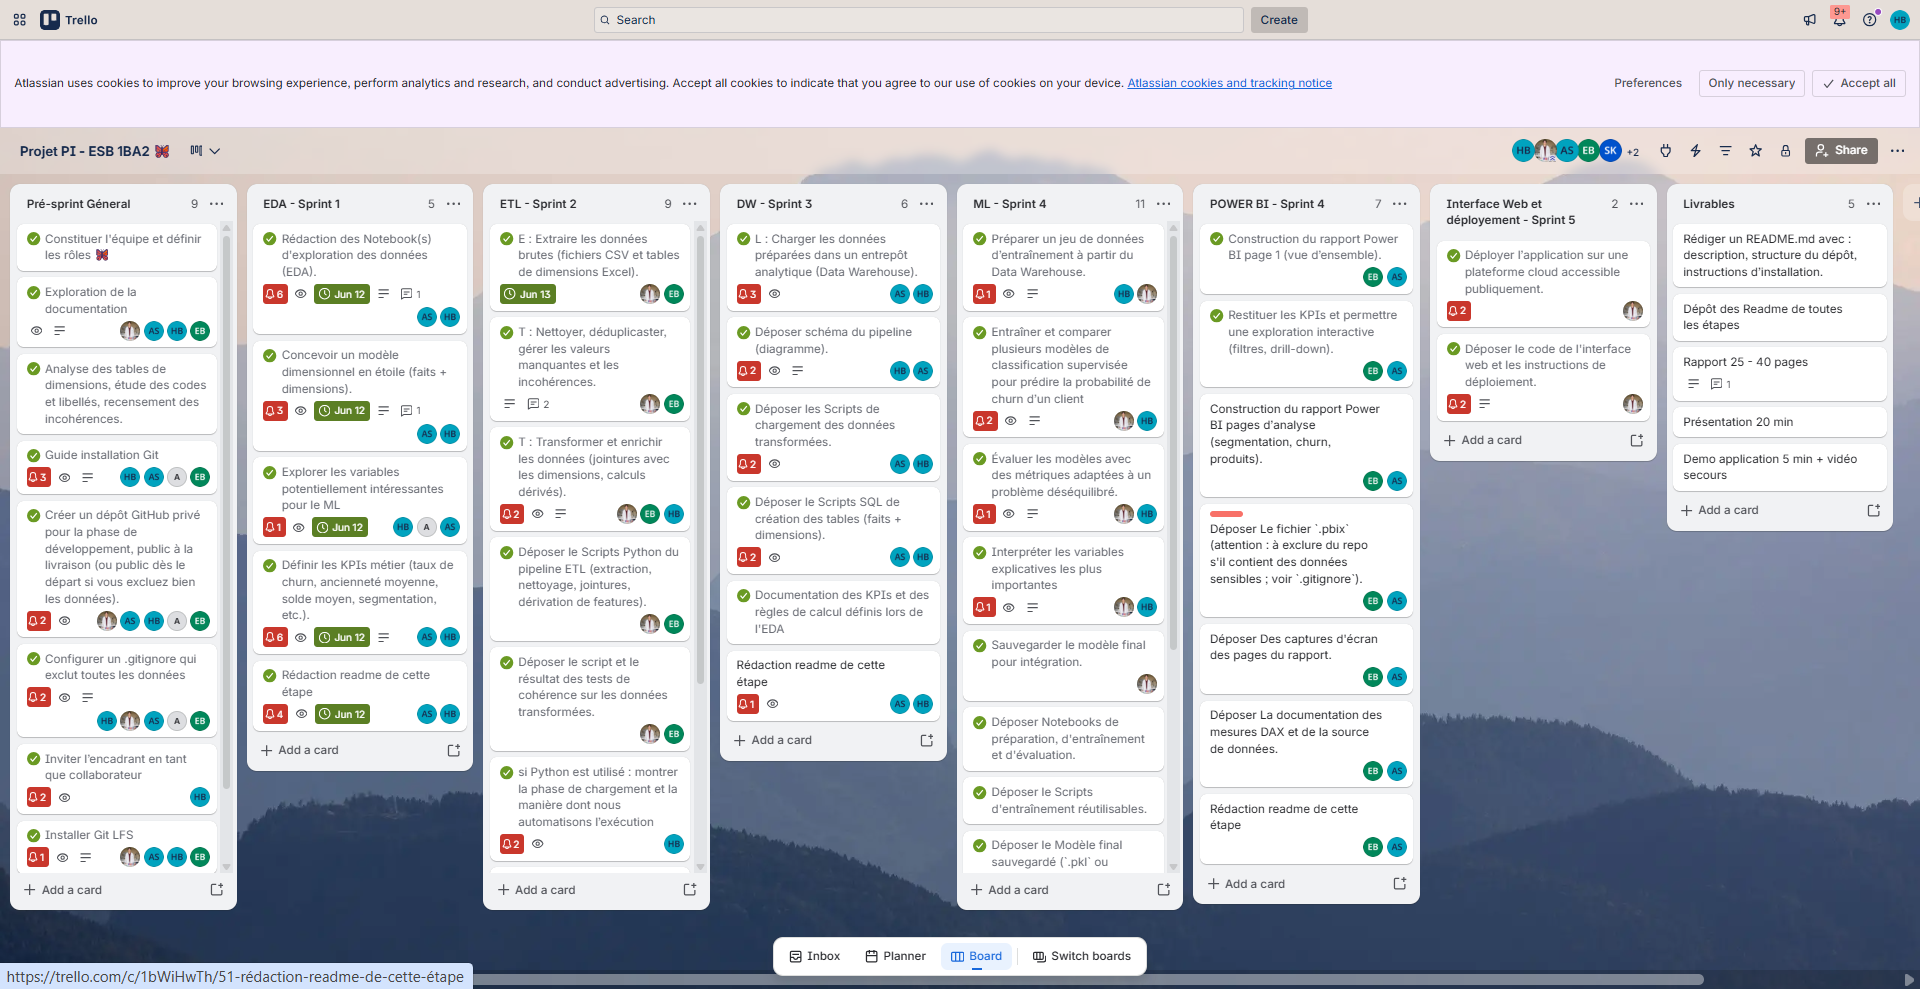
\includegraphics[width=0.95\linewidth]{images/trello_board.png}
	\caption{Tableau Trello de suivi des sprints du projet}
	\label{fig:trello}
\end{figure}
\section{Plan du rapport}

Ce rapport suit l'ordre du pipeline de traitement de la donn\'ee~: description
et exploration des donn\'ees (chapitre~\ref{ch:donnees}), architecture de la
solution (chapitre~\ref{ch:architecture}), ETL et mod\'elisation dimensionnelle
(chapitre~\ref{ch:etl}), tableaux de bord Power BI (chapitre~\ref{ch:powerbi}),
mod\'elisation supervis\'ee (chapitre~\ref{ch:ml}), analyse non supervis\'ee
(chapitre~\ref{ch:datamining}), application web (chapitre~\ref{ch:webapp}),
limites et perspectives (chapitre~\ref{ch:limites}), puis conclusion
(chapitre~\ref{ch:conclusion}).

% ================================================================
% CHAPITRE 2 - DONNEES
% ================================================================
\chapter{Description et exploration des donn\'ees}
\label{ch:donnees}

\section{Origine et anonymisation}

Le jeu de donn\'ees source provient d'un extrait r\'eel d'un syst\`eme
d'information bancaire, anonymis\'e avant transmission \`a l'\'equipe~: tous les
codes internes propri\'etaires ont \'et\'e renomm\'es, les identifiants clients et
comptes remplac\'es par des s\'equences (\texttt{C000001}, \texttt{A0000001}...),
les agences renum\'erot\'ees al\'eatoirement, et la date de naissance r\'eduite \`a
l'ann\'ee. Aucune information directement identifiante (nom, email, t\'el\'ephone,
IBAN) n'est pr\'esente. Le script d'anonymisation (\texttt{anonymize.py}) est
fourni avec le d\'ep\^ot pour tra\c{c}abilit\'e.

\section{Volum\'etrie et grain}

Le fichier source (\texttt{data\_churn.txt}) contient \textbf{528~883 lignes et
34 colonnes}, au grain \'ev\'enement (une ligne par produit rattach\'e \`a un
compte). Huit fichiers de r\'ef\'erentiel Excel (\texttt{dim\_*.xlsx})
compl\`etent le jeu de donn\'ees~: cat\'egories de compte, devises, motifs de
cl\^oture, secteurs d'activit\'e, segments cibles, transactions.

Apr\`es nettoyage (chapitre~\ref{ch:etl}), le jeu de donn\'ees se r\'eduit \`a
\textbf{445~803 \'ev\'enements}, correspondant \`a \textbf{410~587 comptes
uniques}, \textbf{319~129 clients uniques} et \textbf{141 agences}.

\section{D\'efinition retenue du churn}

Le churn est d\'efini au grain \textbf{compte}~: \texttt{churn = 1} si
\texttt{ACCOUNT\_STATUS == "Closed"}. Cette d\'efinition est propag\'ee au grain
\'ev\'enement (chaque ligne li\'ee \`a un compte ferm\'e h\'erite de \texttt{churn=1}),
ce qui produit deux taux de churn selon le grain d'observation~:

\begin{itemize}
\item \textbf{36,1\%} au grain compte (410~587 comptes) - le taux de
      r\'ef\'erence utilis\'e pour la mod\'elisation supervis\'ee
      (chapitre~\ref{ch:ml}).
\item \textbf{41,2\%} au grain \'ev\'enement (445~803 lignes) - plus \'elev\'e
      car les comptes ferm\'es ont, en moyenne, un nombre de produits associ\'es
      l\'eg\`erement diff\'erent des comptes actifs.
\end{itemize}

Pour l'analyse non supervis\'ee au grain client (chapitre~\ref{ch:datamining}),
une d\'efinition alternative a \'et\'e retenue~: \texttt{churn = 1} si et
seulement si \emph{tous} les comptes du client sont ferm\'es (agr\'egation par
\texttt{min} plut\^ot que par \texttt{max}), ce qui \'evite de consid\'erer comme
churn\'e un client ayant simplement ferm\'e un compte secondaire tout en gardant
une relation active avec la banque.

\section{Qualit\'e des donn\'ees - constats de l'exploration}

L'exploration initiale (notebook \texttt{01\_exploration.ipynb}) a mis en
\'evidence plusieurs probl\`emes de qualit\'e, tous document\'es et trait\'es dans
l'\'etape ETL~:

\begin{itemize}
\item \textbf{38~640 doublons stricts} (lignes identiques sur toutes les
      colonnes), supprim\'es.
\item \textbf{44~440 lignes sans num\'ero de compte (\texttt{ACCOUNT\_NO})}
      (8,4\% du fichier d\'edoublonn\'e), jug\'ees inexploitables et supprim\'ees.
\item Des \textbf{dates aberrantes} (ann\'ees de naissance ant\'erieures \`a
      1900, dates d'ouverture post\'erieures aux dates de cl\^oture) - retrait\'e
      au cas par cas (voir section~\ref{sec:bugs-etl}).
\item Des \textbf{valeurs extr\^emes de salaire} (jusqu'\`a 25 millions de
      TND), incompatibles avec les profils clients concern\'es - confirm\'ees
      comme erreurs de saisie et neutralis\'ees.
\item Des \textbf{valeurs manquantes structurelles} sur \texttt{ACCT\_BALANCE}
      et \texttt{SALARY}, volontairement conserv\'ees (non impos\'ees) faute
      d'une m\'ethode d'imputation fiable au vu de l'asym\'etrie des
      distributions.
\end{itemize}

Ces constats ont directement guid\'e les r\`egles de nettoyage impl\'ement\'ees
dans \texttt{01\_etl/etl\_pipeline/clean.py}, d\'etaill\'ees au
chapitre~\ref{ch:etl}.

% ================================================================
% CHAPITRE 3 - ARCHITECTURE
% ================================================================
\chapter{Architecture de la solution}
\label{ch:architecture}

\section{Vue d'ensemble du pipeline}

La solution est organis\'ee en six \'etapes s\'equentielles, chacune consommant
la sortie de la pr\'ec\'edente~:

\begin{center}
\begin{tabular}{c}
Fichier source (\texttt{data\_churn.txt} + \texttt{dim\_*.xlsx}) \\
$\big\downarrow$ \\
ETL (Python / pandas) \\
$\big\downarrow$ \\
Entrep\^ot de donn\'ees (PostgreSQL, sch\'ema en \'etoile) \\
$\big\downarrow$ \\
\begin{tabular}{cc}
Tableaux de bord (Power BI) & Mod\'elisation (scikit-learn / XGBoost)
\end{tabular}\\
$\big\downarrow$ \\
Application web de scoring (Streamlit)
\end{tabular}
\end{center}

Chaque \'etape est ind\'ependante et peut \^etre r\'eex\'ecut\'ee isol\'ement~: le
pipeline ETL expose une fonction \texttt{run\_pipeline()} r\'eutilisable en
m\'emoire (sans n\'ecessiter PostgreSQL), sur laquelle s'appuient \`a la fois les
notebooks de machine learning et de datamining lorsqu'aucune base n'est
accessible.

\section{Choix technologiques}

\begin{center}
\begin{tabularx}{\linewidth}{lX}
\toprule
\textbf{Composant} & \textbf{Technologie retenue et justification} \\
\midrule
Traitement des donn\'ees & Python + pandas - traitement vectoris\'e, code
  versionn\'e et testable (voir comparaison Talend vs Python,
  section~\ref{sec:talend}) \\
Entrep\^ot de donn\'ees & PostgreSQL - SGBD relationnel open source,
  contraintes d'int\'egrit\'e r\'ef\'erentielle natives \\
Visualisation d\'ecisionnelle & Power BI Desktop - impos\'e par le cahier des
  charges \\
Machine learning & scikit-learn~\citep{pedregosa2011sklearn} + XGBoost~\citep{chen2016xgboost} 
  + imbalanced-learn (SMOTE,~\citealp{chawla2002smote}) \\
Application web & Streamlit - prototypage rapide d'une interface data
  science sans d\'eveloppement front-end s\'epar\'e \\
\bottomrule
\end{tabularx}
\end{center}

\section{Sch\'ema en \'etoile}

Le mod\`ele dimensionnel retenu suit la m\'ethodologie de
Kimball~\citep{kimball2013}~: une table de faits centrale
(\texttt{fact\_account\_event}, au grain \'ev\'enement compte$\times$produit) reli\'ee
\`a six tables de dimension~:

\begin{center}
\begin{tabular}{ll}
\toprule
\textbf{Dimension} & \textbf{Contenu} \\
\midrule
\texttt{dim\_client}   & Attributs client (\^age, statut marital, segment, score KYC...) \\
\texttt{dim\_account}  & Attributs compte (cat\'egorie, devise, statut, motif de cl\^oture) \\
\texttt{dim\_branch}   & Agence \\
\texttt{dim\_product}  & Ligne/groupe de produit, au grain contrat \\
\texttt{dim\_date}     & Calendrier (jour, mois, trimestre, ann\'ee) \\
\texttt{dim\_closure}  & Motif de cl\^oture, classifi\'e volontaire/involontaire \\
\bottomrule
\end{tabular}
\end{center}

Toutes les cl\'es de substitution (\emph{surrogate keys}) sont des cha\^ines de
caract\`eres pr\'efix\'ees et num\'erot\'ees (\texttt{CLI\_000001},
\texttt{DATE\_00001}, \texttt{ACC\_0000001}...), avec une largeur de
z\'ero-remplissage calcul\'ee dynamiquement selon le volume de chaque dimension
- ce choix facilite la lecture des cl\'es en base et \'evite toute ambigu\"it\'e
avec un identifiant m\'etier num\'erique.

% ================================================================
% CHAPITRE 4 - ETL ET DATA WAREHOUSE
% ================================================================
\chapter{ETL et mod\'elisation dimensionnelle}
\label{ch:etl}

\section{Pipeline ETL}

Le pipeline ETL est impl\'ement\'e en Python (module \texttt{01\_etl/etl\_pipeline/}),
orchestr\'e en cinq \'etapes s\'equentielles~: \texttt{extract} (lecture du CSV et
des r\'ef\'erentiels Excel), \texttt{clean} (r\`egles de nettoyage), 
\texttt{dimensions} (construction des tables de dimension et de leurs cl\'es),
\texttt{fact} (construction de la table de faits), \texttt{load} (chargement
PostgreSQL via SQLAlchemy). Un script de test de coh\'erence ind\'ependant
(\texttt{test\_coherence\_donnees.py}, 32~tests r\'epartis en 5~cat\'egories -
compl\'etude, domaine, inter-colonnes, temporel, cardinalit\'e) valide le
r\'esultat sans modifier le pipeline lui-m\^eme.

\subsection{Anomalies r\'eelles d\'ecouvertes et corrig\'ees}
\label{sec:bugs-etl}

Sept anomalies concr\`etes ont \'et\'e identifi\'ees en testant le pipeline contre
les donn\'ees r\'eelles, document\'ees avec leur nombre exact de lignes
concern\'ees~:

\begin{enumerate}
\item \textbf{\texttt{MARITAL\_STATUS} incoh\'erent pour 25 lignes} (personnes
      morales) - la r\`egle de correction ne s'appliquait qu'aux valeurs
      manquantes, laissant passer des valeurs d\'ej\`a pr\'esentes et
      incoh\'erentes avec un statut de personne morale.
\item \textbf{\texttt{ACCT\_OPENING\_DATE} post\'erieure \`a
      \texttt{ACCT\_CLOSE\_DATE}} (33~571 lignes) - pollution confirm\'ee par
      des dates proches de l'extraction du fichier source, neutralis\'ees en
      valeur manquante plut\^ot que conserv\'ees fausses.
\item \textbf{\texttt{STARTDATE} post\'erieure \`a \texttt{MATURITYDATE}}
      (2~575 lignes) - m\^eme m\'ecanisme, corrig\'e de la m\^eme mani\`ere.
\item \textbf{Jointure sur cl\'e nulle} (\texttt{dim\_Closure\_reason}) -
      une valeur nulle c\^ot\'e r\'ef\'erentiel produisait un produit cart\'esien et
      des doublons en cascade.
\item \textbf{Encodage UTF-8 non forc\'e} sous Windows/psycopg2 - corrig\'e
      en imposant explicitement \texttt{client\_encoding=utf8}.
\item \textbf{Coercition enti\`ere impr\'evue} sur \texttt{date\_key} lors du
      chargement - r\'esolue par le passage \`a des cl\'es textuelles plut\^ot
      que num\'eriques (voir ci-dessous).
\item \textbf{D\'ependance de cl\'e \'etrang\`ere \`a la relance} - PostgreSQL
      refusait de supprimer une dimension tant que la table de faits la
      r\'ef\'eren\c{c}ait encore~; corrig\'e en supprimant syst\'ematiquement la
      table de faits avant toute op\'eration sur les dimensions.
\end{enumerate}

\subsection{V\'erification de la nullit\'e structurelle de \texttt{date\_key}}

\texttt{date\_key} est la seule cl\'e \'etrang\`ere de la table de faits pour
laquelle une valeur manquante est normale~: elle d\'erive de
\texttt{ACCT\_OPENING\_DATE}, volontairement conserv\'ee \`a vide pour certains
comptes. Un contr\^ole explicite a \'et\'e ajout\'e au pipeline~: le nombre de
\texttt{date\_key} manquants doit \^etre strictement \'egal au nombre
d'\texttt{ACCT\_OPENING\_DATE} manquantes en amont. V\'erifi\'e contre les
donn\'ees r\'eelles~: \textbf{134~056 lignes (30,1\%)}, exactement \'egal - confirmant
une nullit\'e enti\`erement structurelle, sans \'echec de jointure r\'eel.

\section{Entrep\^ot de donn\'ees PostgreSQL}

Le chargement dans PostgreSQL a \'et\'e valid\'e sur un serveur r\'eel~: les 7
tables (6 dimensions + 1 table de faits) se chargent avec succ\`es et toutes
les contraintes de cl\'e \'etrang\`ere s'appliquent sans erreur. La
figure~\ref{fig:postgres-dw} montre le r\'esultat d'une requ\^ete d'inspection
sur \texttt{dim\_account} via pgAdmin, confirmant la structure des cl\'es
textuelles et la coh\'erence des donn\'ees charg\'ees.

\begin{figure}[H]
\centering
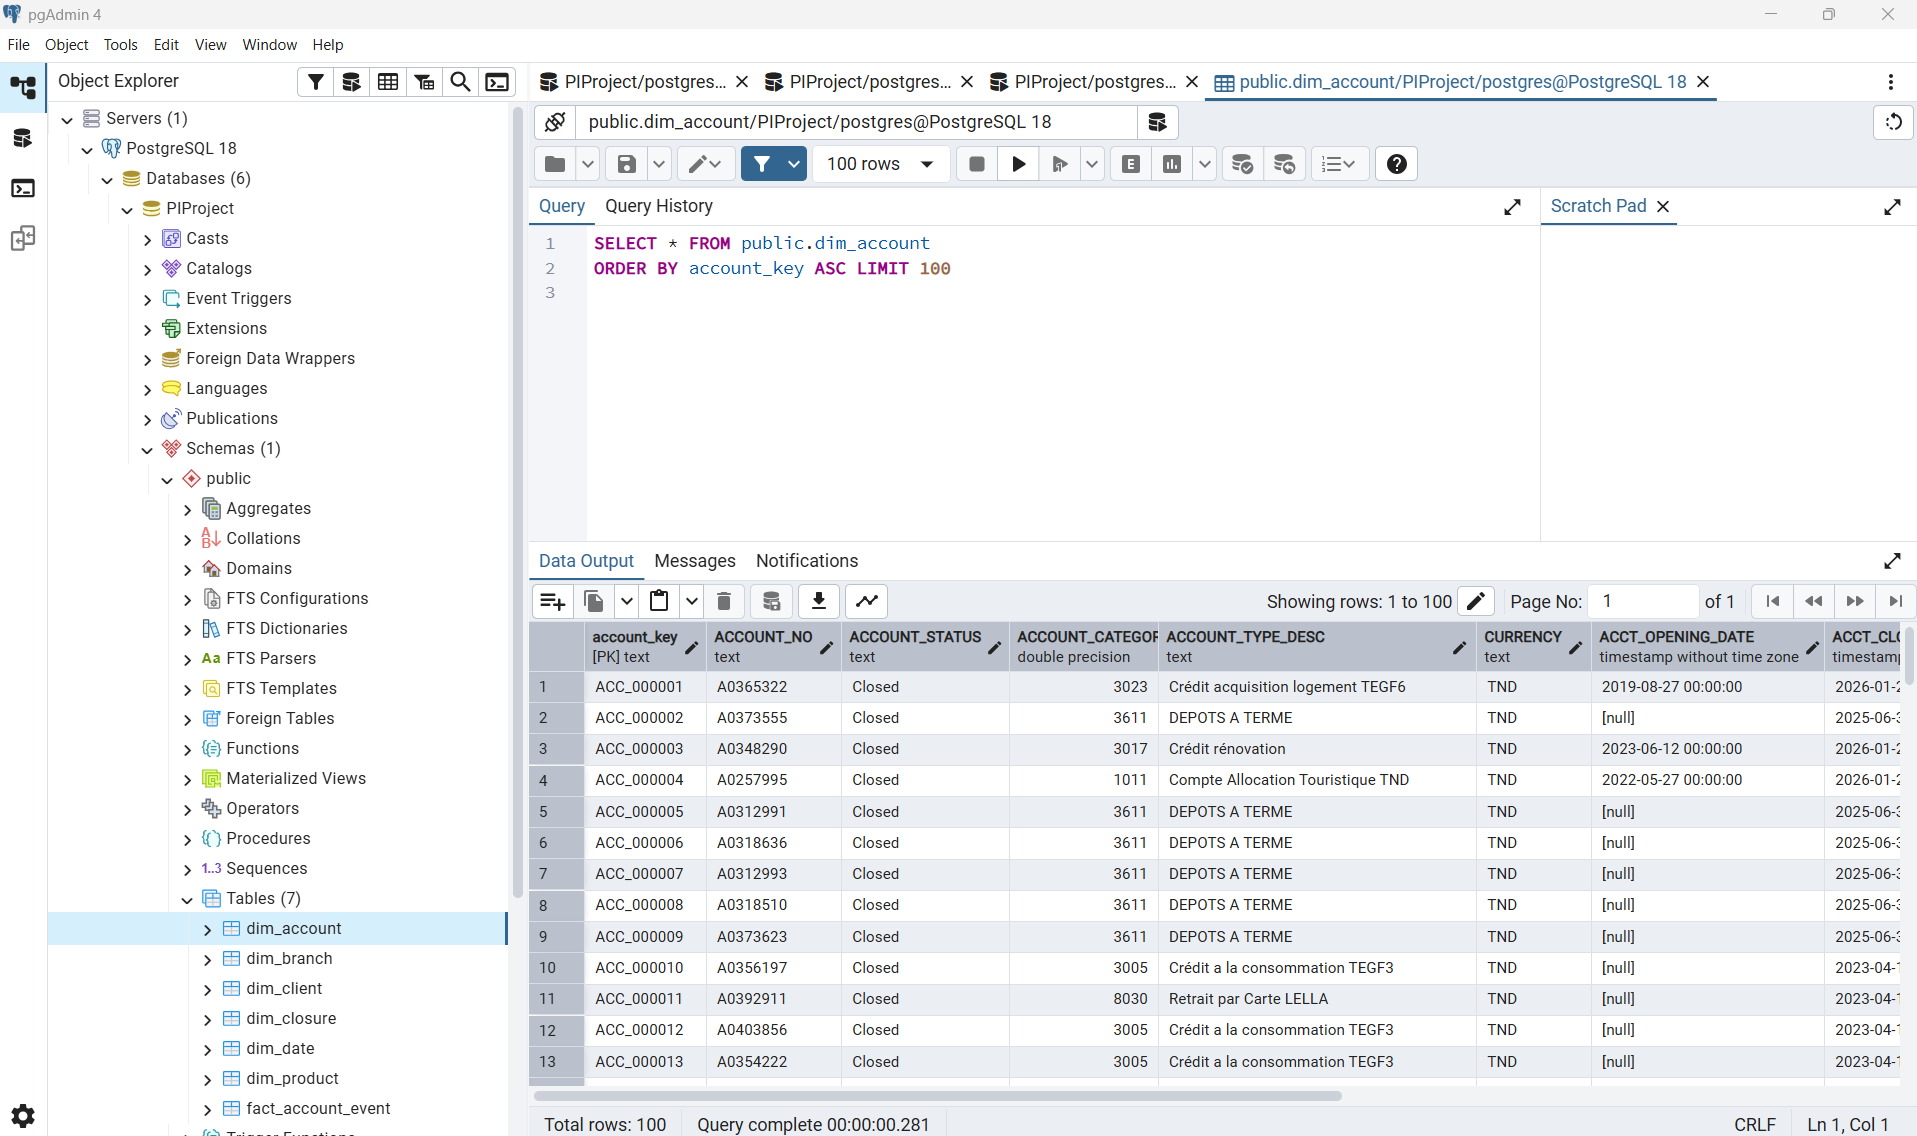
\includegraphics[width=0.92\linewidth]{images/postgres_dw.png}
\caption{Entrep\^ot de donn\'ees PostgreSQL - inspection de \texttt{dim\_account} via pgAdmin (chargement r\'eel valid\'e, 7/7 tables)}
\label{fig:postgres-dw}
\end{figure}

\section{Comparaison Talend vs Python}
\label{sec:talend}

Une question r\'ecurrente en soutenance concerne le choix d'un pipeline codé en
Python plut\^ot qu'un outil ETL graphique tel que Talend Open
Studio~\citep{talenddocs}, plus classique dans un cursus Business Analytics.
Le tableau~\ref{tab:talend} r\'esume la comparaison, fond\'ee sur l'exp\'erience
r\'eelle de ce projet (7 bugs trouv\'es et corrig\'es en cours de route).

\begin{table}[H]
\centering
\small
\begin{tabularx}{\linewidth}{lXX}
\toprule
\textbf{Crit\`ere} & \textbf{Talend Open Studio} & \textbf{Python (pandas)} \\
\midrule
Courbe d'apprentissage & Interface visuelle, prise en main rapide pour des
  transformations simples & N\'ecessite de coder, mais l'\'equipe le ma\^itrisait
  d\'ej\`a \\
Tra\c{c}abilit\'e Git & Jobs stock\'es en XML propri\'etaire compil\'e, diff
  illisible & Chaque r\`egle m\'etier est un \texttt{git diff} de quelques
  lignes, lisible en revue de code \\
D\'ebogage & D\'ebogueur visuel, mais isole mal une transformation pr\'ecise sur
  528~883 lignes & Isolation directe d'une colonne/condition en une commande
  pandas - ainsi trouv\'es les 7 bugs r\'eels \\
Tests automatis\'es & Difficile \`a int\'egrer nativement & Chaque \'etape est une
  fonction testable unitairement (32 tests \'ecrits) \\
Installation & Lourde (JDK, IDE $\sim$1--2~Go) & L\'eg\`ere (\texttt{pip
  install}) \\
Connecteurs & Nombreux, sans code & Couverture native CSV/Excel/PostgreSQL via
  pandas/SQLAlchemy \\
Approche visuelle & Flux visible d'un coup d'\oe il & Flux lin\'eaire dans le
  code, document\'e par un diagramme et ce rapport \\
\bottomrule
\end{tabularx}
\caption{Comparaison Talend Open Studio vs pipeline Python}
\label{tab:talend}
\end{table}

\textbf{Choix retenu~:} Python. Le facteur d\'ecisif a \'et\'e la tra\c{c}abilit\'e
Git pour un travail d'\'equipe \`a cinq avec relecture de code, et la
possibilit\'e d'\'ecrire des tests automatis\'es qui ont concr\`etement r\'ev\'el\'e
3 des 7 bugs corrig\'es. L'inconvenient assum\'e - moins imm\'ediatement lisible
pour un public non technique en soutenance - est compens\'e par un diagramme
du sch\'ema et la documentation \'ecrite du pipeline.

% ================================================================
% CHAPITRE 5 - POWER BI
% ================================================================
\chapter{Analyses BI et tableaux de bord Power BI}
\label{ch:powerbi}

Conform\'ement au cahier des charges, le rapport Power BI est construit en
trois pages minimum, connect\'ees directement \`a l'entrep\^ot de donn\'ees
PostgreSQL~\citep{powerbidocs}~: une vue d'ensemble, une analyse du profil
client, et une analyse du risque financier associ\'e au churn.

\section{Vue d'ensemble}

La page d'accueil pr\'esente les indicateurs cl\'es~: taux de churn global
(41,16\%, coh\'erent avec le taux pond\'er\'e par \'ev\'enement calcul\'e dans le
pipeline ETL), nombre de clients distincts (319K, coh\'erent avec
\texttt{dim\_client}), taux de r\'etention (58,84\%), et la Value-at-Risk (VaR)
associ\'ee au churn (5,42~milliards de TND). Un graphique combin\'e retrace
l'\'evolution annuelle du nombre de churns et sa croissance ann\'ee sur ann\'ee.

\begin{figure}[H]
\centering
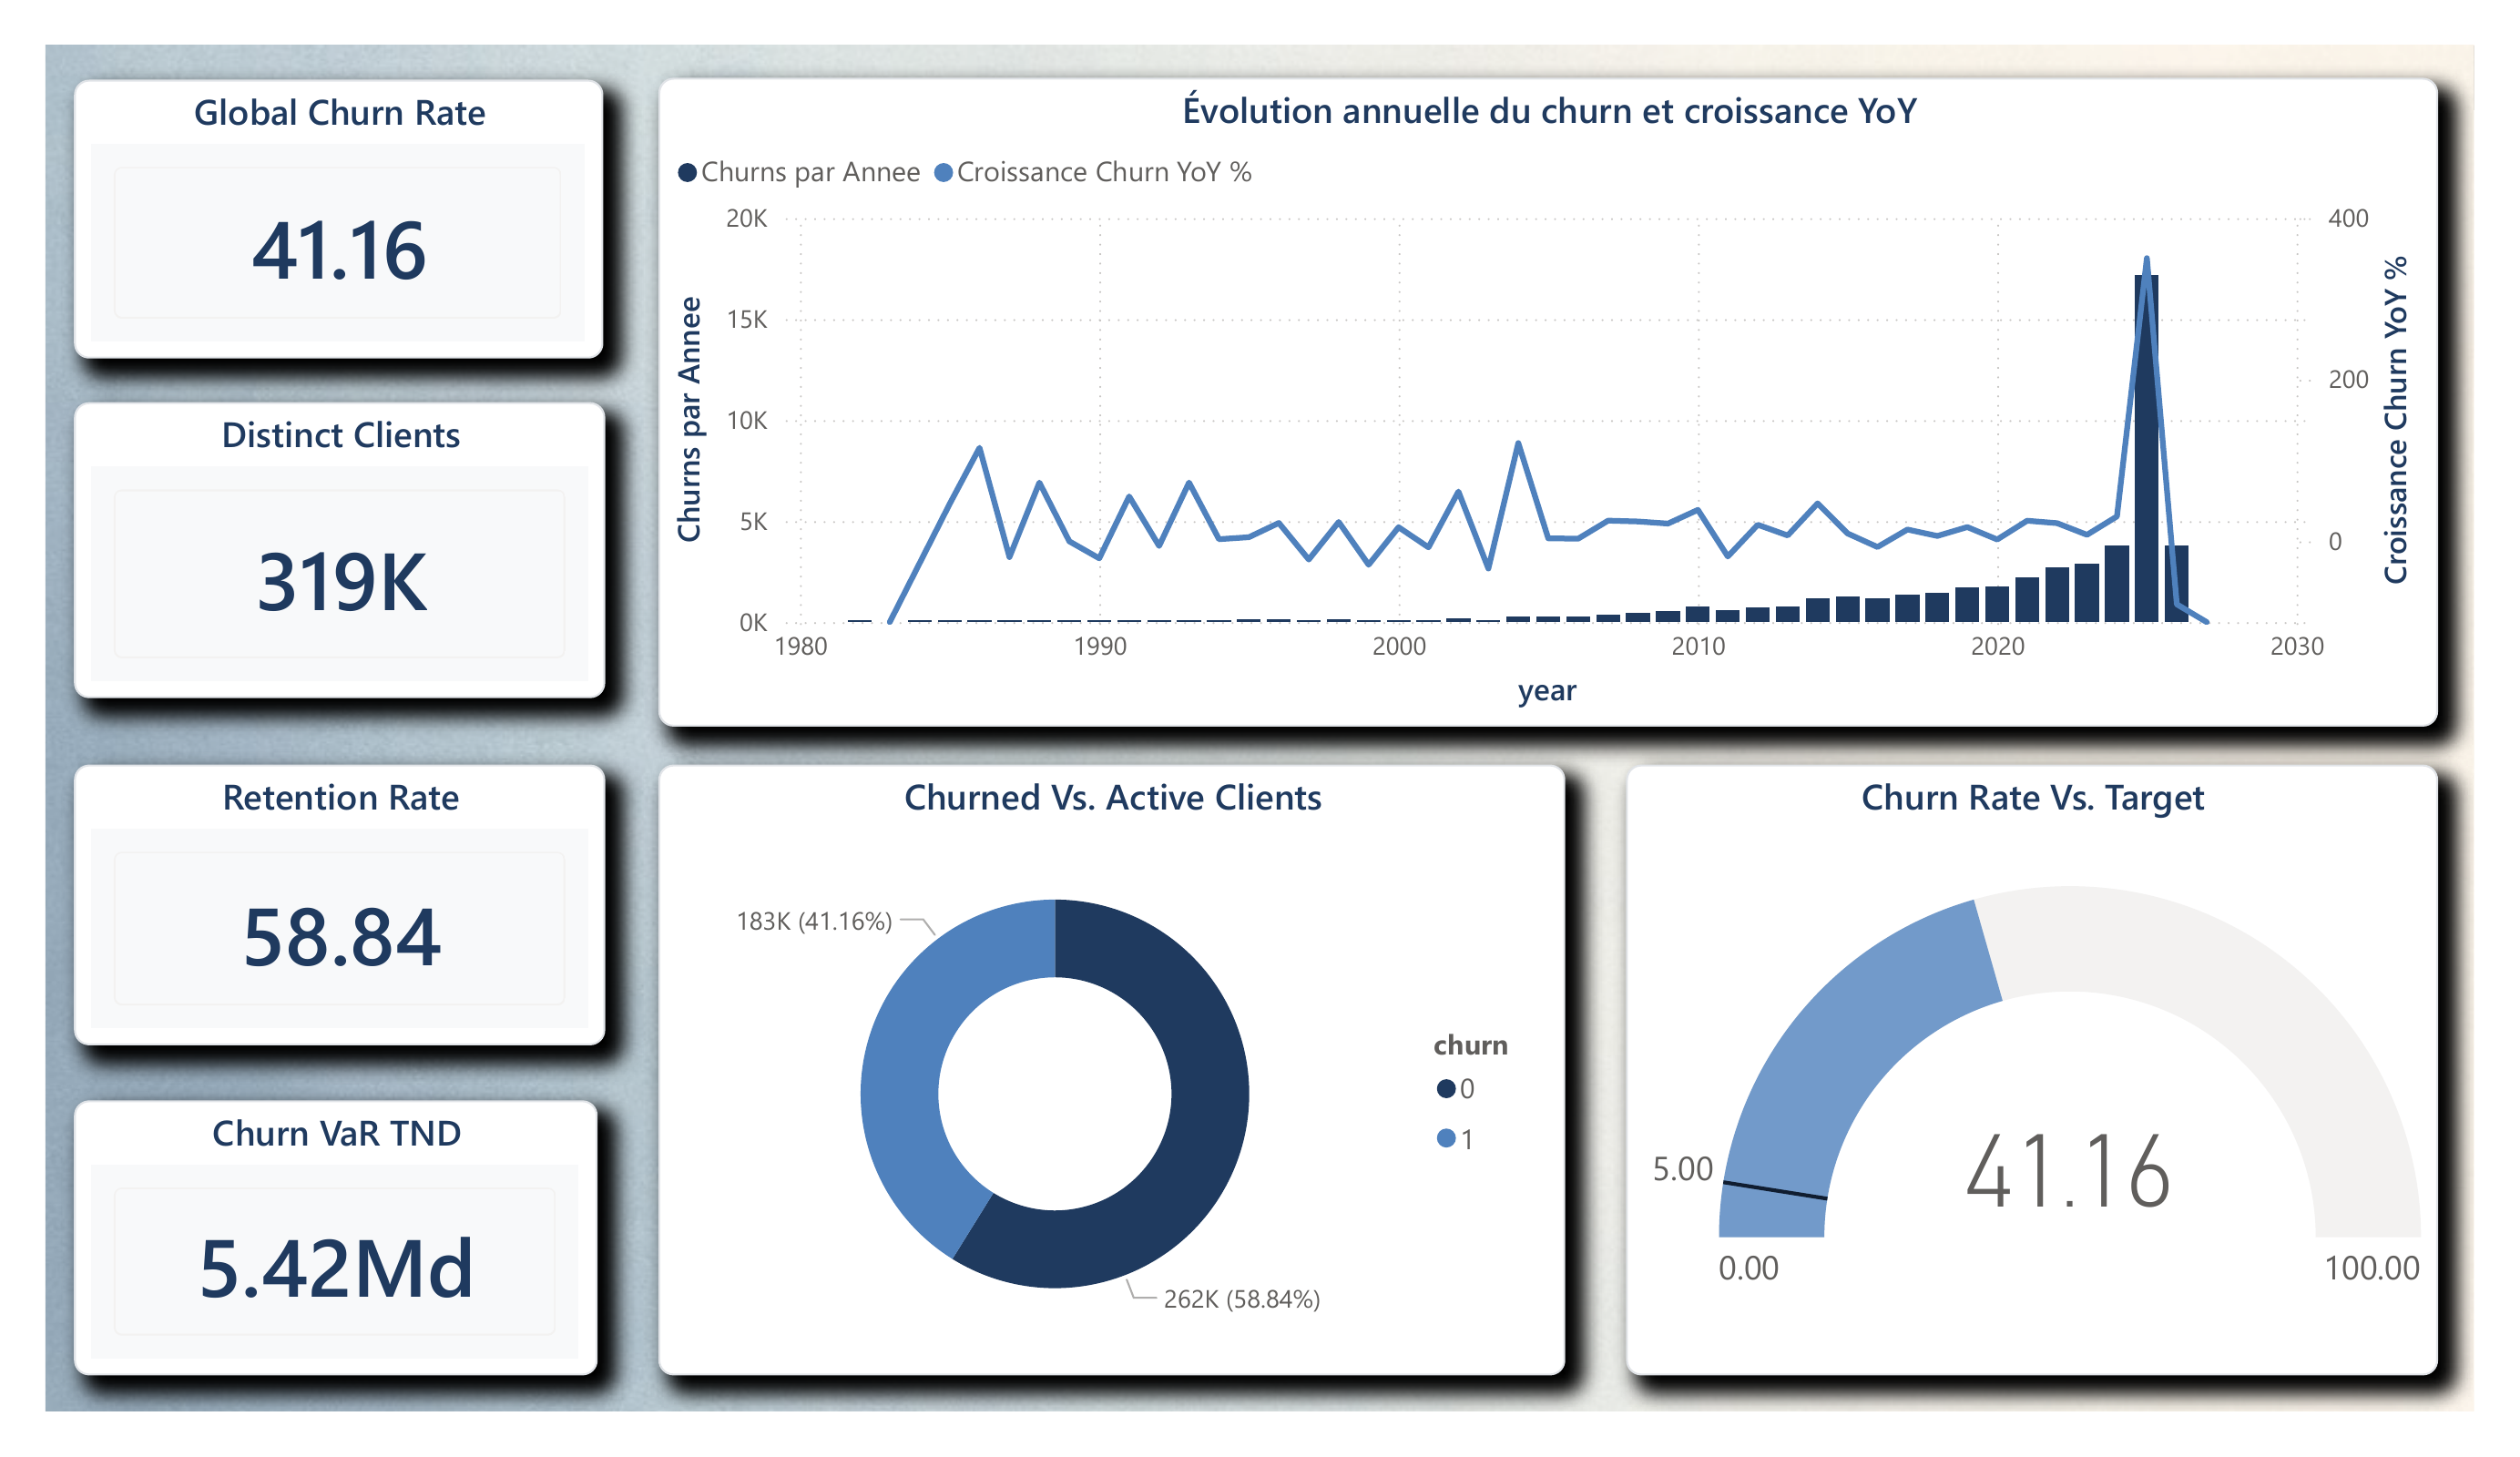
\includegraphics[width=0.95\linewidth]{images/powerbi_overview.png}
\caption{Vue d'ensemble - taux de churn global, r\'etention, \'evolution annuelle et VaR}
\label{fig:powerbi-overview}
\end{figure}

\section{Analyse du profil client}

La deuxi\`eme page d\'ecompose le taux de churn par profil~: \^age, statut
marital, score KYC et segment (\texttt{PARTYCLASS}), avec des filtres
interactifs permettant de croiser ces dimensions. Le graphique salaire moyen
churn\'e vs actif fait appara\^itre un \'ecart marqu\'e - les clients churn\'es
ayant en moyenne un salaire inf\'erieur aux clients actifs sur le segment
observ\'e.

\begin{figure}[H]
\centering
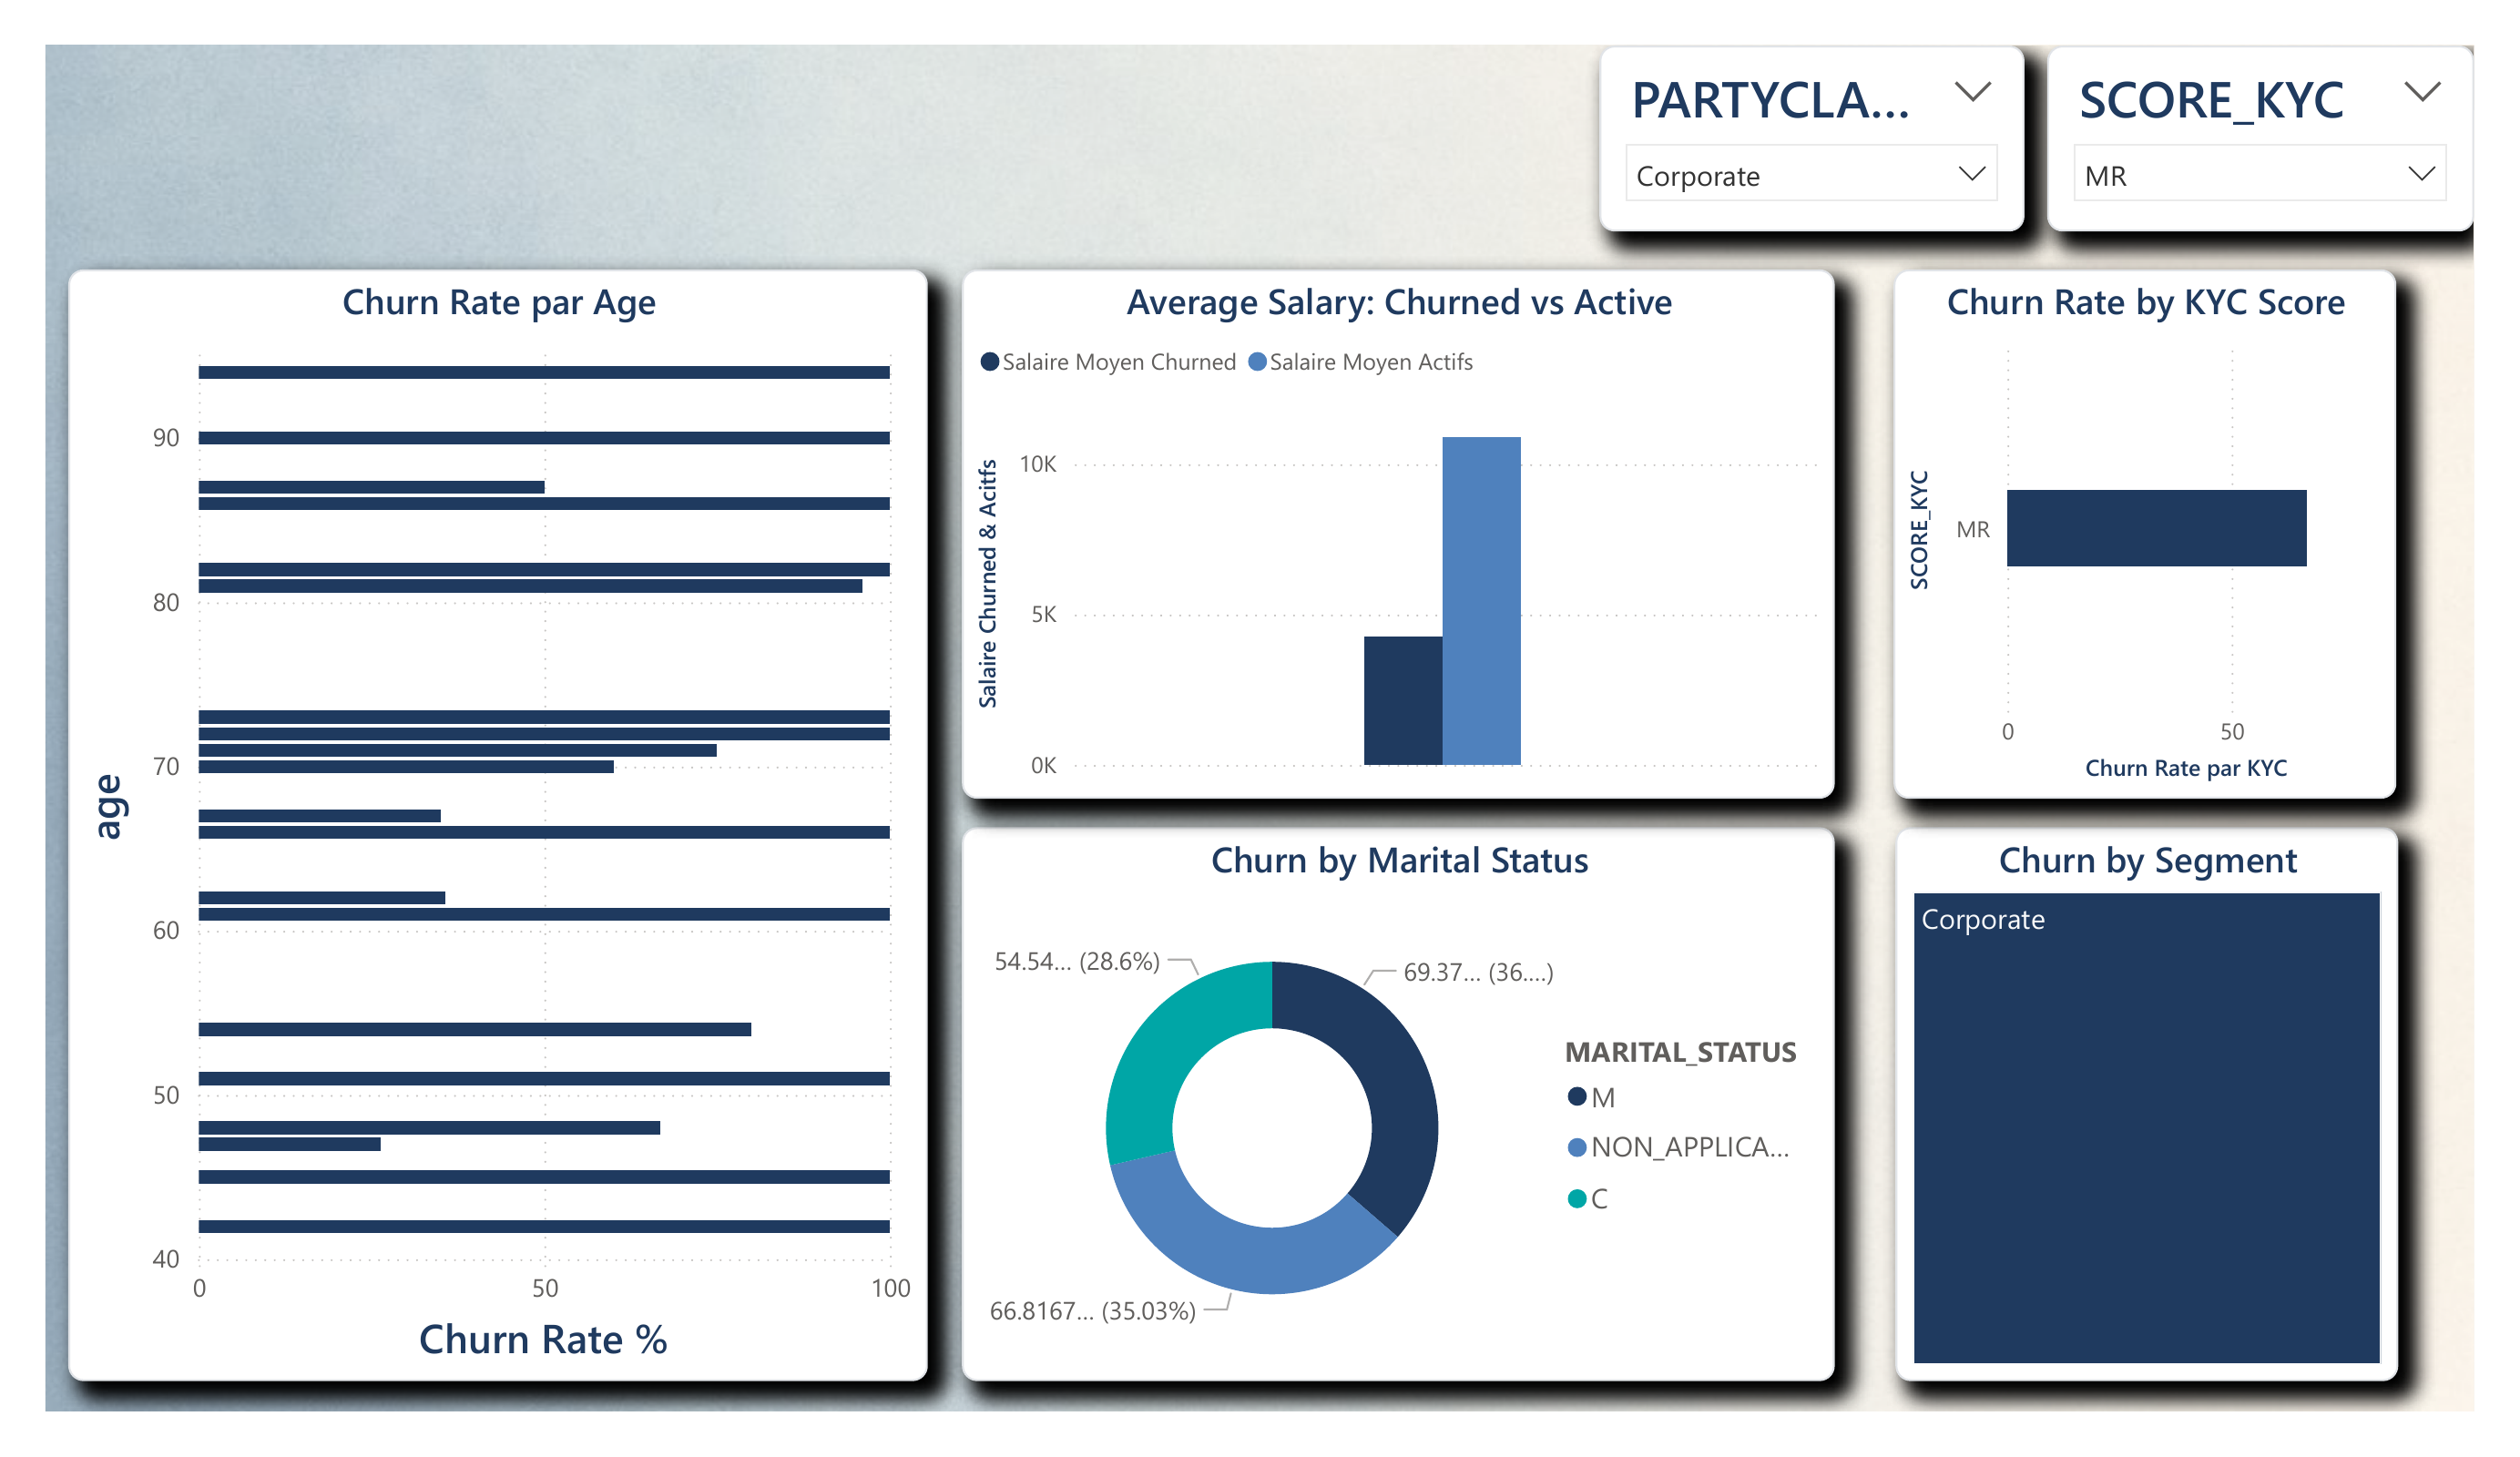
\includegraphics[width=0.95\linewidth]{images/powerbi_profil.png}
\caption{Analyse du churn par profil client (\^age, statut marital, score KYC, segment)}
\label{fig:powerbi-profil}
\end{figure}

\section{Analyse produits et risque financier}

La troisi\`eme page explore la relation entre le nombre de produits d\'etenus
et le taux de churn (une courbe en cloche, le churn augmentant fortement puis
se stabilisant \`a un plateau proche de 100\% au-del\`a d'un certain seuil de
produits), ainsi que la r\'epartition churn\'e/actif par ligne de produit -
les d\'ep\^ots (\texttt{DEPOSITS}) affichant le taux de churn le plus \'elev\'e
(95,71\%), coh\'erent avec leur nature de produits \`a \'ech\'eance.

\begin{figure}[H]
\centering
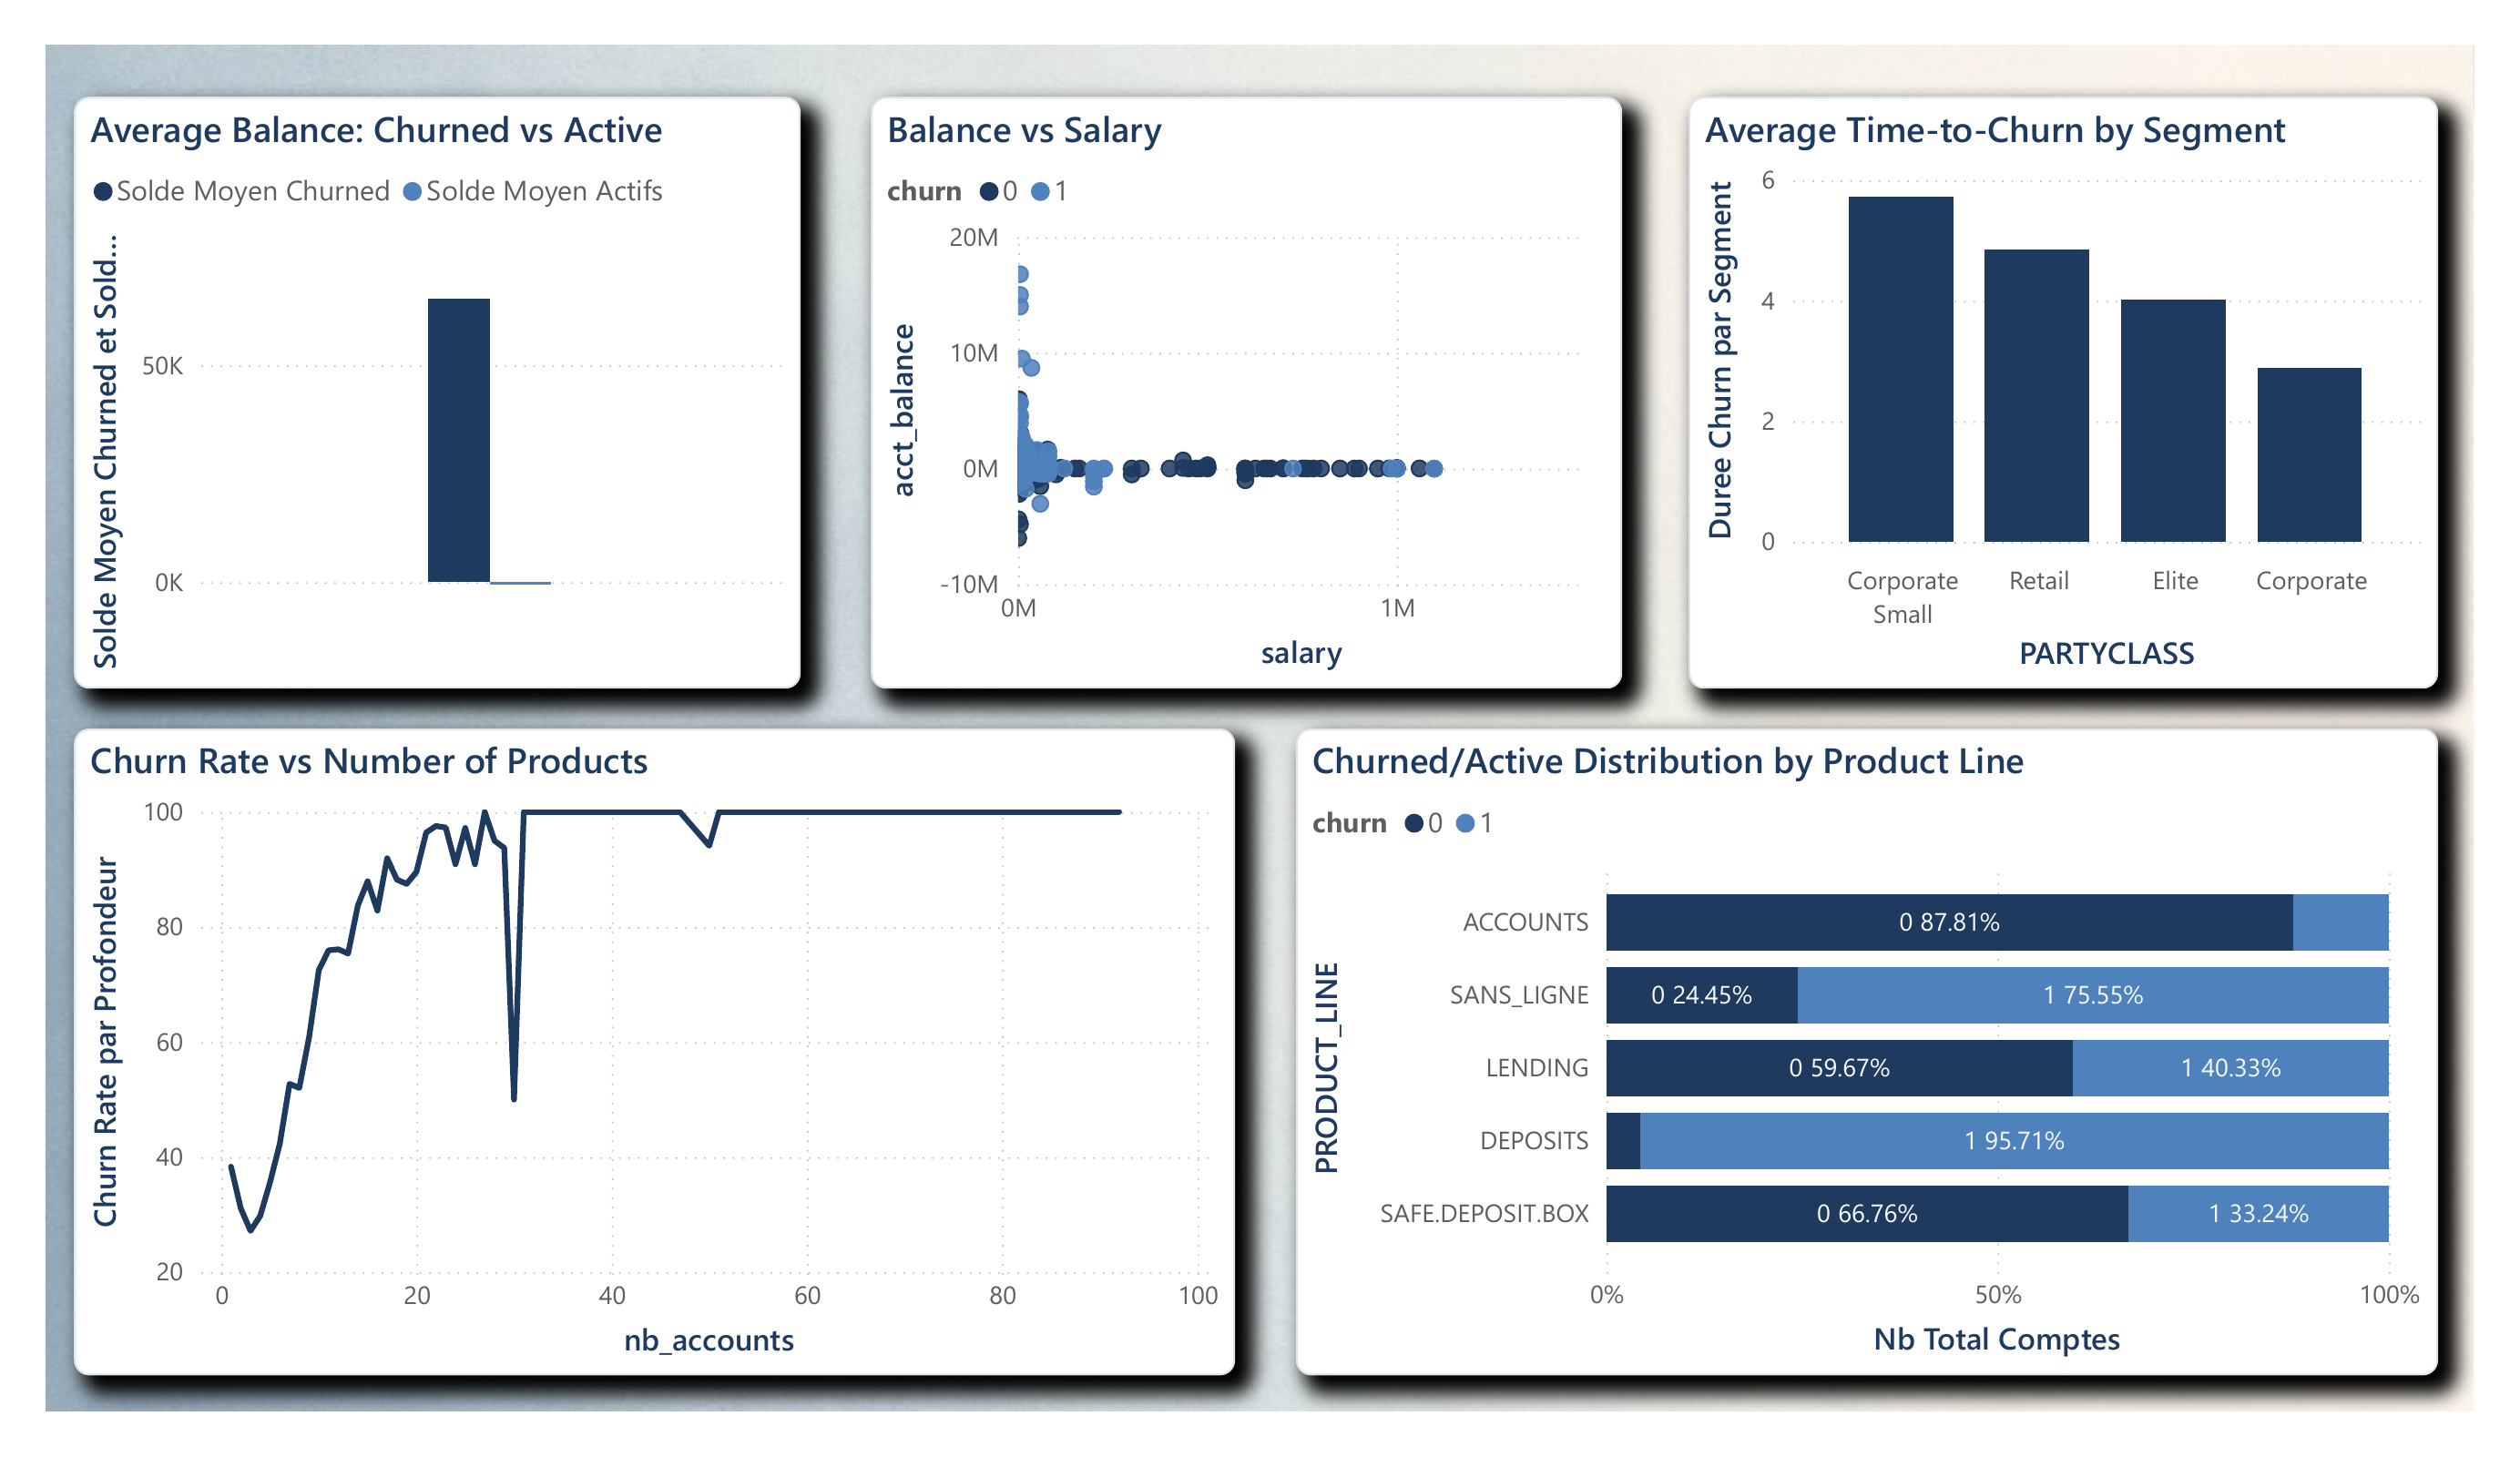
\includegraphics[width=0.95\linewidth]{images/powerbi_produits.png}
\caption{Analyse du risque par produit - solde, dur\'ee avant churn, r\'epartition par ligne de produit}
\label{fig:powerbi-produits}
\end{figure}

\section{D\'ecomposition de la Value-at-Risk (VaR)}

Une page compl\'ementaire d\'ecompose la VaR totale li\'ee au churn (54,08
millions de TND sur le p\'erim\`etre filtr\'e) par segment (\texttt{PARTYCLASS}),
ligne de produit et score KYC, \`a travers une visualisation en flux
(\emph{decomposition tree}) permettant \`a un analyste m\'etier d'explorer
librement les contributeurs au risque. Une matrice de risque
(segment~$\times$~score KYC) compl\`ete cette analyse avec un score de risque
brut par cellule.

\begin{figure}[H]
\centering
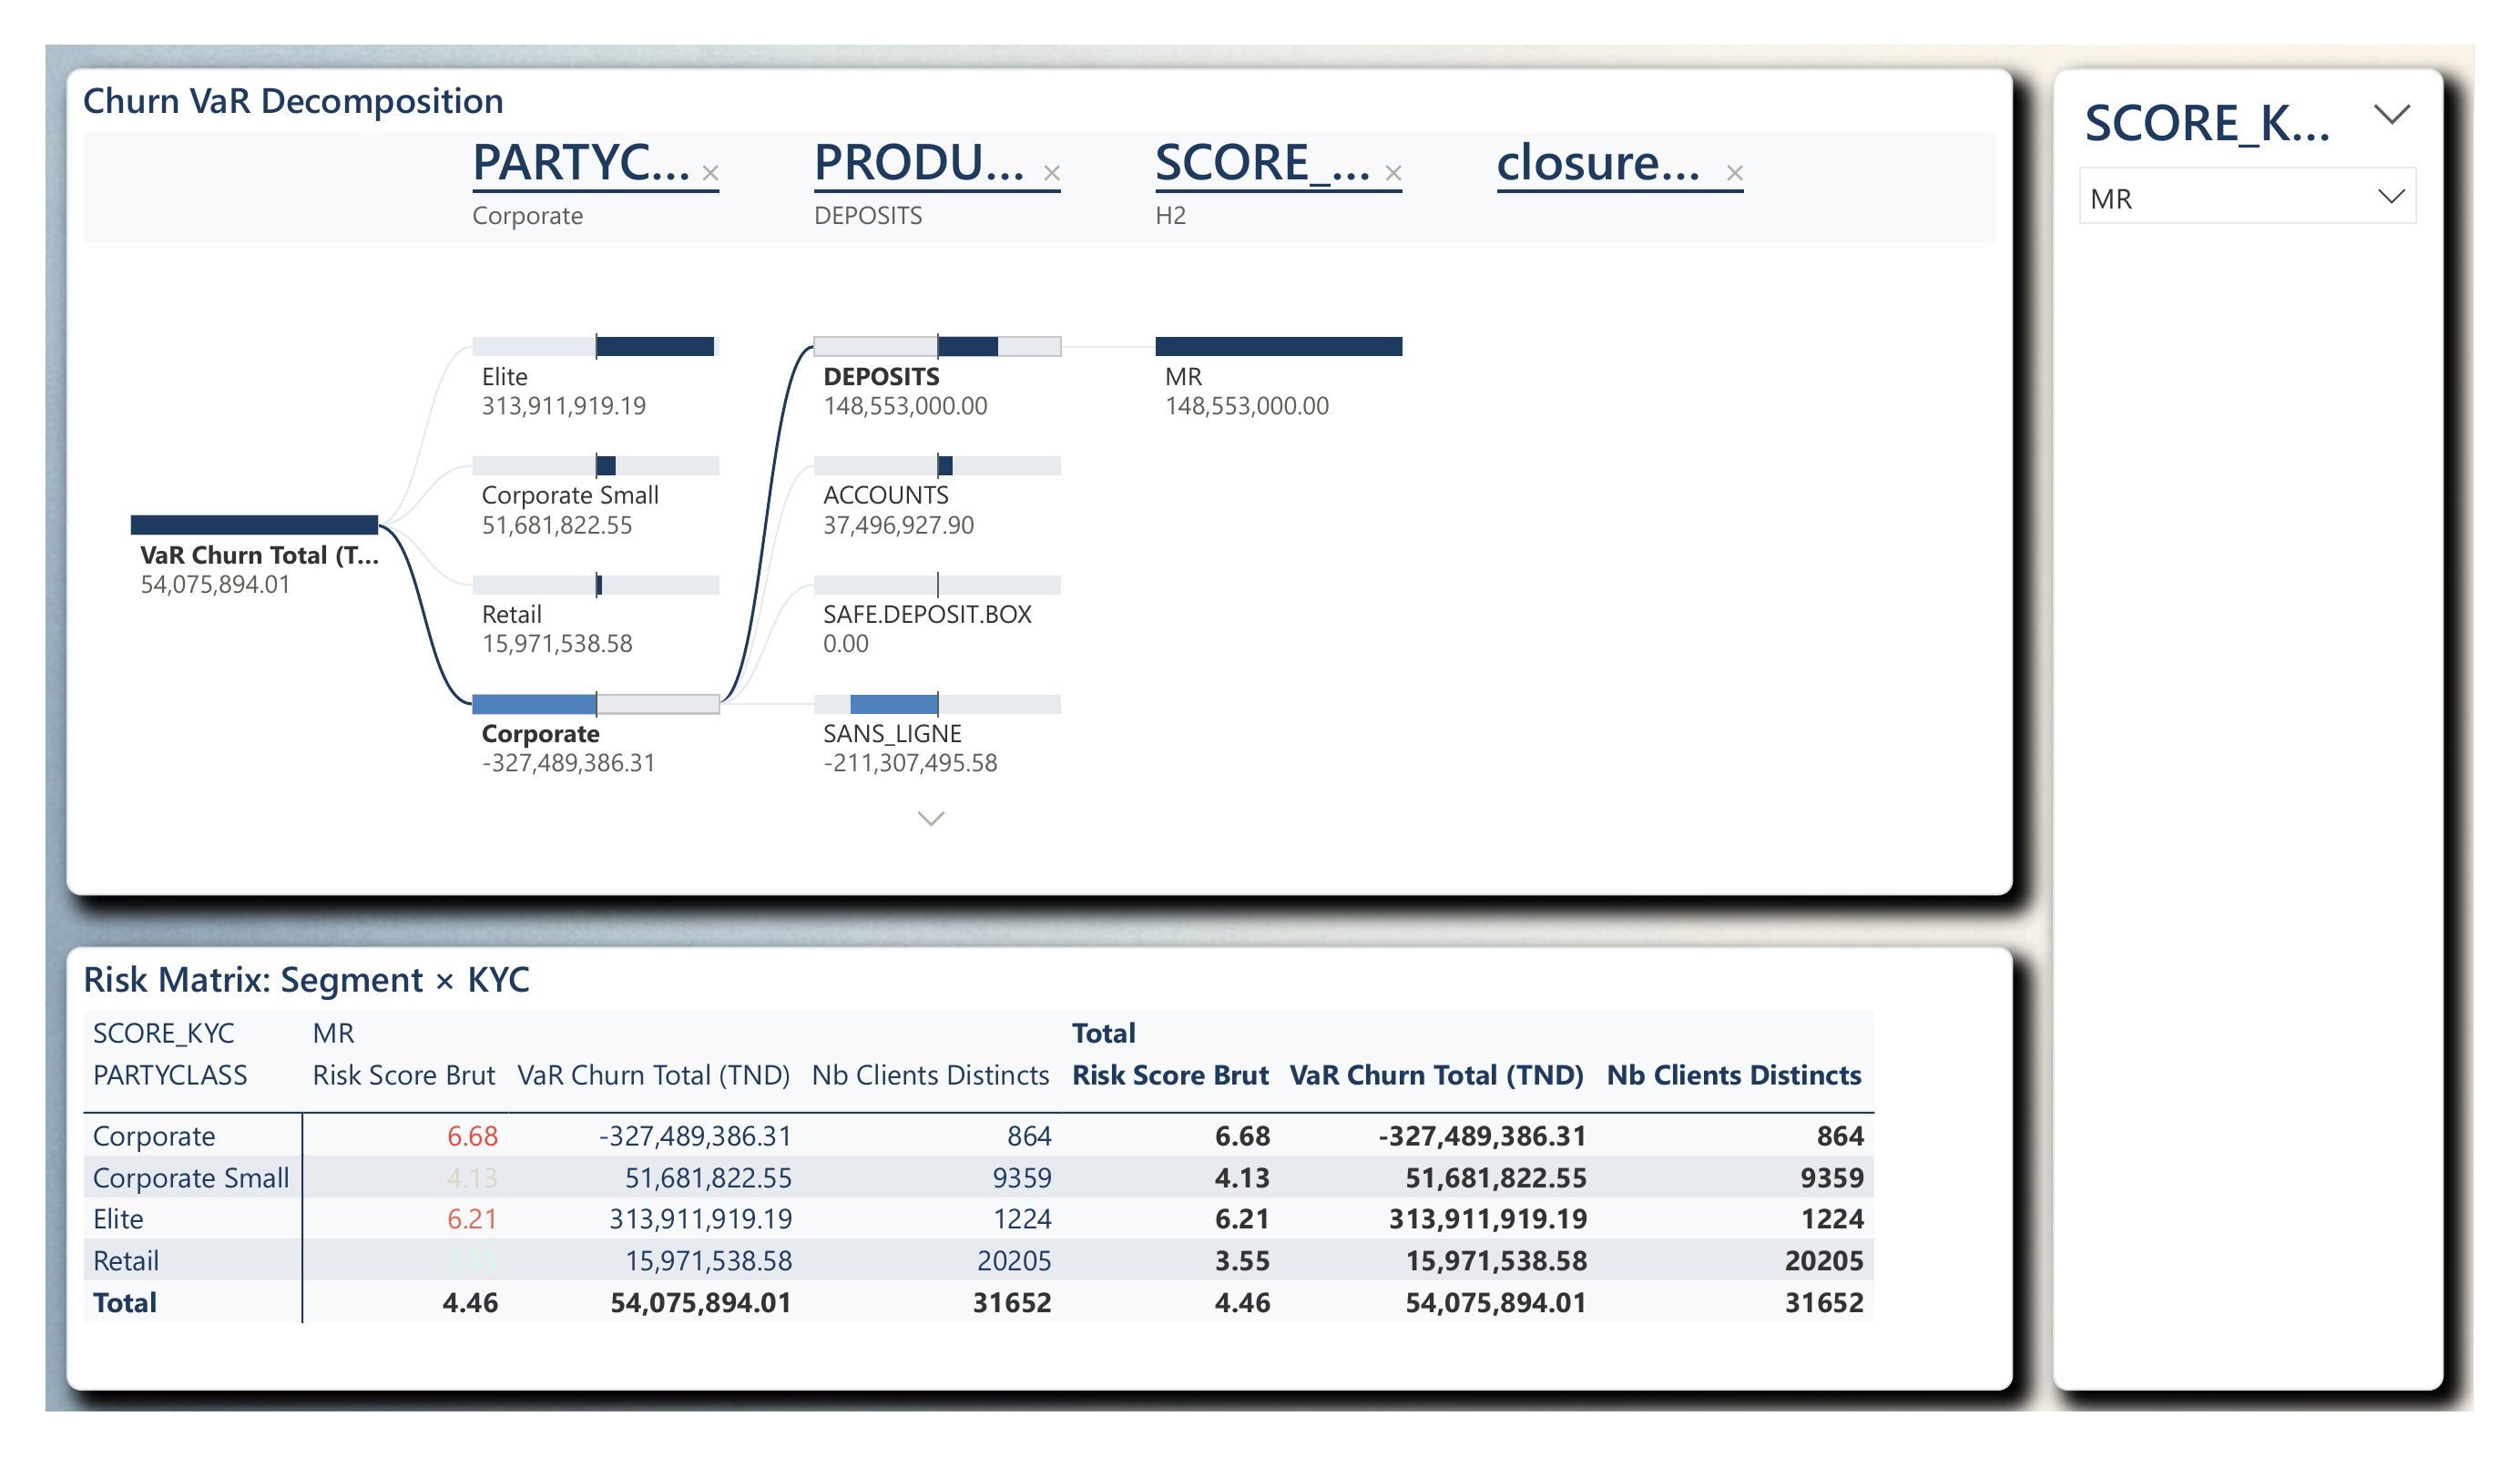
\includegraphics[width=0.95\linewidth]{images/powerbi_var.png}
\caption{D\'ecomposition de la Value-at-Risk du churn par segment, produit et score KYC}
\label{fig:powerbi-var}
\end{figure}

\section{Limites de cette partie}

La d\'ecomposition de la VaR fait appara\^itre des valeurs n\'egatives pour
certaines branches (ex.\ segment \texttt{Corporate}~: $-327,5$ millions de
TND), signalant que la mesure DAX sous-jacente combine des flux de signe
oppos\'e (probablement solde net positif et n\'egatif agr\'eg\'es) - un point \`a
clarifier avec l'\'equipe avant toute utilisation d\'ecisionnelle de cet
indicateur en l'\'etat.

% ================================================================
% CHAPITRE 6 - MACHINE LEARNING
% ================================================================
\chapter{Mod\'elisation supervis\'ee - pr\'ediction du churn}
\label{ch:ml}

\section{Grain et p\'erim\`etre}

Le mod\`ele supervis\'e est entra\^in\'e au grain \textbf{compte}
(\texttt{ACCOUNT\_NO}), conform\'ement \`a la d\'efinition officielle du churn
(section~\ref{ch:donnees}). La table de faits (grain \'ev\'enement) est agr\'eg\'ee
par compte avant tout entra\^inement, ce qui ram\`ene le jeu de donn\'ees \`a
410~587 lignes.

\section{S\'election des variables}

Chaque variable exclue l'a \'et\'e pour une raison document\'ee individuellement
dans le notebook~: variables de fuite \'evidentes
(\texttt{ACCT\_CLOSE\_DATE}, \texttt{CLOSURE\_REASON}, \texttt{ACCOUNT\_STATUS}
- directement d\'eriv\'ees du label), identifiants
(\texttt{account\_key}, \texttt{client\_key}, \texttt{branch\_key}), variables
redondantes (\texttt{ACCOUNT\_TYPE\_DESC}, quasi identique \`a
\texttt{ACCOUNT\_CATEGORY}) et variables quasi constantes
(\texttt{NATIONALITY}, \texttt{RESIDENCE}, $>$93\% de la m\^eme valeur).

\section{Fuite de donn\'ees d\'etect\'ee et corrig\'ee}
\label{sec:leakage}

Un point m\'ethodologique important m\'erite d'\^etre document\'e en d\'etail~: une
premi\`ere version du notebook cr\'eait des indicateurs binaires de valeur
manquante (\texttt{\_missing}) pour chaque variable pr\'esentant des absences.
L'analyse d'importance des variables d'XGBoost a alors r\'ev\'el\'e que
\texttt{acct\_tenure\_days\_missing} repr\'esentait \textbf{89,5\%} du poids de
d\'ecision du mod\`ele - un chiffre anormalement \'elev\'e ayant d\'eclench\'e une
v\'erification.

La cause a \'et\'e confirm\'ee~: la correction de nettoyage \'evoqu\'ee \`a la
section~\ref{sec:bugs-etl} (neutralisation d'\texttt{ACCT\_OPENING\_DATE}
lorsqu'elle est post\'erieure \`a \texttt{ACCT\_CLOSE\_DATE}) ne s'applique qu'\`a
des comptes d\'ej\`a ferm\'es - rendant la nullit\'e r\'esultante de
\texttt{acct\_tenure\_days} un quasi-proxy parfait du label \`a pr\'edire (100\%
des comptes concern\'es sont \texttt{Closed}, v\'erifi\'e empiriquement), et non un
signal m\'etier l\'egitime.

Les indicateurs \texttt{acct\_tenure\_days\_missing} et
\texttt{acct\_balance\_missing} ont donc \'et\'e retir\'es des variables
explicatives. \texttt{salary\_missing} a \'et\'e conserv\'e apr\`es v\'erification
qu'il s'agit bien d'un signal l\'egitime (taux de churn quasi identique,
$\sim$37\% vs $\sim$35\%, que le salaire soit renseign\'e ou non). Le F1-score
d'XGBoost n'a quasiment pas chang\'e apr\`es correction (0,9465 contre 0,9460
avant), confirmant que le mod\`ele disposait d\'ej\`a de signaux l\'egitimes
suffisants.

\begin{quote}
Cette d\'ecouverte illustre une le\c{c}on m\'ethodologique g\'en\'erale~: toujours
v\'erifier qu'une performance apparente n'est pas un artefact du pipeline de
nettoyage amont avant de faire confiance \`a un r\'esultat de mod\'elisation.
\end{quote}

\section{Pr\'etraitement}

Les variables cat\'egorielles \`a faible cardinalit\'e sont encod\'ees en
\emph{one-hot}~; \texttt{ACCOUNT\_CATEGORY} (149 valeurs) et
\texttt{BRANCH} (141 valeurs) sont encod\'ees par fr\'equence, ajust\'ee
uniquement sur l'ensemble d'entra\^inement pour \'eviter toute fuite. Le jeu de
donn\'ees est s\'epar\'e 80/20 de mani\`ere stratifi\'ee, et SMOTE~\citep{chawla2002smote}
est appliqu\'e uniquement sur l'ensemble d'entra\^inement pour r\'e\'equilibrer les
classes.

\section{Mod\`eles compar\'es et r\'esultats}

Six mod\`eles ont \'et\'e entra\^in\'es et compar\'es~: r\'egression logistique
(r\'ef\'erence), K plus proches voisins (KNN), arbre de d\'ecision, for\^et
al\'eatoire~\citep{breiman2001random}, machine \`a vecteurs de support (SVM) et
XGBoost~\citep{chen2016xgboost}.

\begin{table}[H]
\centering
\begin{tabular}{lccl}
\toprule
\textbf{Mod\`ele} & \textbf{F1-score} & \textbf{ROC-AUC} & \textbf{Remarques} \\
\midrule
R\'egression logistique & 0,6963 & 0,8015 & Mod\`ele de r\'ef\'erence \\
KNN & $\sim$0,87 & $\sim$0,95 & \'Evalu\'e sur 10K lignes de test (co\^ut de pr\'ediction) \\
Arbre de d\'ecision & 0,9438 & 0,9758 & \texttt{max\_depth=10} \\
For\^et al\'eatoire & 0,9329 & 0,9772 & 200 arbres \\
SVM & $\sim$0,70 & $\sim$0,85 & 20K lignes d'entra\^inement (co\^ut noyau RBF) \\
\textbf{XGBoost} & \textbf{0,9465} & \textbf{0,9823} & \textbf{Mod\`ele retenu} \\
\bottomrule
\end{tabular}
\caption{Comparaison des mod\`eles de classification (grain compte, apr\`es correction de la fuite de donn\'ees)}
\label{tab:ml-results}
\end{table}

L'effet de SMOTE s'est av\'er\'e marginal sur ce jeu de donn\'ees - le
d\'es\'equilibre des classes (64\%/36\%) \'etant mod\'er\'e plut\^ot qu'extr\^eme.
L'analyse d'importance des variables d'XGBoost (apr\`es correction de la fuite)
identifie \texttt{amount\_total} (40,5\%), \texttt{nb\_produits} (27,2\%) et
\texttt{acct\_tenure\_days} (16,4\%) comme les trois variables les plus
influentes.

\section{Limitations assum\'ees}

KNN est \'evalu\'e sur un sous-\'echantillon de 10~000 comptes de test (la
pr\'ediction sur le jeu complet prend $\sim$150 secondes, jug\'e
disproportionn\'e). SVM est entra\^in\'e sur un sous-\'echantillon de 20~000
comptes (sur 328~469 disponibles), le co\^ut du noyau RBF rendant
l'entra\^inement sur le jeu complet trop co\^uteux. Ces limitations sont
document\'ees explicitement dans le notebook pour \'eviter toute comparaison \`a
armes rigoureusement \'egales entre ces deux mod\`eles et les quatre autres.

% ================================================================
% CHAPITRE 7 - DATAMINING NON SUPERVISE
% ================================================================
\chapter{Analyse non supervis\'ee - segmentation et anomalies}
\label{ch:datamining}

\section{Motivation et grain}

La mod\'elisation supervis\'ee (chapitre~\ref{ch:ml}) r\'epond \`a une question
binaire~: \emph{ce compte va-t-il churner ?}. Elle ne dit rien, en revanche,
sur les profils clients sous-jacents ni sur l'existence de comportements
atypiques ne correspondant \`a aucun segment standard. Une analyse
compl\'ementaire non supervis\'ee a donc \'et\'e men\'ee, \`a un grain diff\'erent~:
le \textbf{client} (et non le compte), avec la d\'efinition du churn agr\'eg\'ee
par \texttt{min} (churn = 1 si et seulement si tous les comptes du client sont
ferm\'es - voir section~\ref{ch:donnees}). Ce grain regroupe
\textbf{319~129 clients}.

\section{Analyse en composantes principales (ACP)}

Les variables quantitatives (\texttt{salary}, \texttt{amount\_total},
\texttt{fixedrate\_mean}, \texttt{nb\_produits}, \texttt{age}) sont
standardis\'ees puis projet\'ees par ACP~\citep{jolliffe2002pca}, apr\`es
transformation logarithmique de \texttt{salary} et transformation
\emph{symlog} de \texttt{amount\_total} (positif et n\'egatif possibles, avec
des valeurs extr\^emes). L'ACP retient 5 composantes~; les deux premi\`eres
expliquent \textbf{54,46\%} de la variance totale (34,37\% + 20,09\%), les
trois premi\`eres \textbf{74,02\%}.

\section{Segmentation par K-means}

Un algorithme K-means \`a $k=4$ est appliqu\'e sur les variables standardis\'ees.
Les quatre segments obtenus sont fortement d\'es\'equilibr\'es en taille~:

\begin{table}[H]
\centering
\begin{tabular}{lrl}
\toprule
\textbf{Cluster} & \textbf{Taille} & \textbf{Profil moyen} \\
\midrule
0 & 125~603 & Salaire moyen (729 TND), peu de produits (1,31), \^age \'elev\'e (62,6 ans) \\
1 &  22~615 & Salaire \'elev\'e (5~098 TND), 3,52 produits, taux fixe moyen \'elev\'e (7,44) \\
2 &      12 & Cas extr\^emes~: \texttt{amount\_total} moyen de 38 milliards, 744 produits en moyenne \\
3 & 170~899 & Profil le plus jeune (36,3 ans), peu de produits (1,13), faible engagement \\
\bottomrule
\end{tabular}
\caption{Segments K-means ($k=4$, grain client, $n=319\,129$)}
\label{tab:kmeans}
\end{table}

Le cluster~2 (12 clients) correspond \`a des valeurs extr\^emes plut\^ot qu'\`a un
v\'eritable segment m\'etier - \`a rapprocher de la d\'etection d'anomalies
ci-dessous plut\^ot qu'\`a interpr\'eter comme une strat\'egie de r\'etention
diff\'erenci\'ee.

\section{D\'etection d'anomalies par Isolation Forest}

Un mod\`ele Isolation Forest~\citep{liu2008isolation} est appliqu\'e sur les
m\^emes variables standardis\'ees pour identifier des clients dont le profil
s'\'ecarte significativement de la distribution g\'en\'erale, ind\'ependamment de
leur appartenance \`a un cluster K-means. \textbf{3~192 clients} (soit environ
1\% de la base) sont signal\'es comme anomalies, dont \textbf{230} appartiennent
au cluster~3 (le segment jeune \`a faible engagement) - sugg\'erant que ce
segment concentre une part disproportionn\'ee de profils atypiques \`a
investiguer manuellement (ex.\ combinaisons rares de solde n\'egatif \'elev\'e et
de peu de produits).

\section{Usage envisag\'e}

Cette analyse non supervis\'ee compl\`ete la pr\'ediction supervis\'ee de deux
mani\`eres~: (1)~elle fournit une base de segmentation exploitable pour cibler
des actions marketing diff\'erenci\'ees par profil, ind\'ependamment du risque de
churn pr\'edit~; (2)~la liste des clients anormaux peut servir de liste de
priorit\'e pour une revue manuelle par un conseiller, en compl\'ement du score
de churn produit par le mod\`ele supervis\'e.

% ================================================================
% CHAPITRE 8 - APPLICATION WEB
% ================================================================
\chapter{Interface web et d\'eploiement}
\label{ch:webapp}

\section{Application Streamlit}

Le mod\`ele retenu (XGBoost, section~\ref{ch:ml}) est restitu\'e via une
application Streamlit~\citep{streamlitdocs} \`a quatre pages~: un \'ecran
d'accueil pr\'esentant un r\'esum\'e du jeu de donn\'ees, un formulaire de
scoring individuel (saisie des caract\'eristiques d'un client/compte et
pr\'ediction en temps r\'eel), un tableau de bord KPI interactif, et une page
de pr\'esentation de l'\'equipe.

Le mod\`ele (\texttt{model.pkl}), l'ordre des colonnes attendues
(\texttt{feature\_columns.pkl}) et l'encodeur de fr\'equence
(\texttt{frequency\_encoder.pkl}) sont s\'erialis\'es et charg\'es au d\'emarrage de
l'application, garantissant que le pr\'etraitement appliqu\'e en production est
strictement identique \`a celui utilis\'e \`a l'entra\^inement.

\section{D\'eploiement}

L'application est con\c{c}ue pour un d\'eploiement sur Streamlit Community
Cloud. \emph{Lien de d\'emonstration~: \`a compl\'eter par l'\'equipe lors du
d\'eploiement final (voir \texttt{05\_web\_app/README.md} du d\'ep\^ot).}

\section{Point de vigilance}

Le mod\`ele charg\'e est li\'e aux features d\'efinies au grain \textbf{compte}
(chapitre~\ref{ch:ml}). Si une \'evolution future du notebook de mod\'elisation
change de grain ou de jeu de variables, \texttt{model.pkl} et
\texttt{feature\_columns.pkl} doivent \^etre r\'eg\'en\'er\'es et remplac\'es dans
\texttt{05\_web\_app/models/}, faute de quoi l'application produirait des
pr\'edictions incoh\'erentes sans erreur explicite.

% ================================================================
% CHAPITRE 9 - LIMITES ET PERSPECTIVES
% ================================================================
\chapter{Limites et perspectives}
\label{ch:limites}

\section{Limites connues}

\begin{itemize}
\item \textbf{Anomalies temporelles non corrig\'ees} (document\'ees mais non
      trait\'ees)~: 53 lignes o\`u \texttt{DATE\_OF\_BIRTH} est post\'erieure \`a
      \texttt{CUST\_OPENING\_DATE}, et 114 lignes o\`u
      \texttt{LAST\_REVIEW\_DATE} est post\'erieure \`a
      \texttt{NEXT\_REVIEW\_DATE} - l'incoh\'erence source ne permet pas de
      d\'eterminer avec certitude laquelle des deux dates est erron\'ee.
\item \textbf{Absence de validation crois\'ee} (k-fold) sur les mod\`eles
      supervis\'es - un seul d\'ecoupage train/test a \'et\'e utilis\'e par souci
      de temps d'ex\'ecution (le pipeline complet prend d\'ej\`a 15 \`a 20
      minutes).
\item \textbf{Absence d'optimisation des hyperparam\`etres}
      (\texttt{GridSearchCV} ou \'equivalent) sur les mod\`eles retenus.
\item \textbf{Absence d'explicabilit\'e par instance} (SHAP) - seule
      l'importance globale des variables est disponible actuellement.
\item \textbf{Incoh\'erences r\'esiduelles entre le notebook narratif et le
      pipeline de production}~: le notebook \'etape par étape
      (\texttt{01\_etl/notbooks ETL/02\_ETL.ipynb}) ne r\'eplique pas encore la
      correction sur \texttt{ACCT\_OPENING\_DATE} appliqu\'ee dans
      \texttt{etl\_pipeline/clean.py}, produisant un taux de nullit\'e de
      \texttt{date\_key} l\'eg\`erement diff\'erent (22,5\% contre 30,1\% en
      production) - \`a harmoniser.
\item \textbf{D\'ecomposition de la VaR Power BI} pr\'esentant des valeurs
      n\'egatives sur certains segments (section~\ref{ch:powerbi}), \`a
      clarifier avant utilisation d\'ecisionnelle.
\end{itemize}

\section{Perspectives}

\begin{itemize}
\item Revue syst\'ematique des corrections ETL pour d'\'eventuels effets de
      bord similaires \`a la fuite de donn\'ees d\'ecrite \`a la
      section~\ref{sec:leakage}.
\item Mise en place d'une validation crois\'ee et d'une recherche
      d'hyperparam\`etres pour affiner encore le mod\`ele XGBoost retenu.
\item Int\'egration de SHAP pour une explicabilit\'e individuelle des
      pr\'edictions, utile en contexte r\'eglementaire bancaire.
\item Rapprochement des r\'esultats de la segmentation K-means
      (chapitre~\ref{ch:datamining}) avec les scores de churn supervis\'es,
      pour construire une matrice risque$\times$valeur client actionnable par
      les conseillers.
\item D\'eploiement effectif de l'application Streamlit et int\'egration du
      lien de d\'emonstration dans la documentation du projet.
\end{itemize}

% ================================================================
% CHAPITRE 10 - CONCLUSION
% ================================================================
\chapter{Conclusion}
\label{ch:conclusion}

Ce projet a permis de construire, valider et documenter une cha\^ine compl\`ete
d'analyse du churn bancaire, de l'exploration d'un jeu de donn\'ees brut
jusqu'\`a une application de scoring d\'eploy\'ee. Chaque \'etape a fait l'objet
d'une v\'erification concr\`ete contre des donn\'ees r\'eelles plut\^ot que
suppos\'ee correcte par construction~: 7 anomalies ETL corrig\'ees et
document\'ees avec leur volum\'etrie exacte, une fuite de donn\'ees d\'etect\'ee et
r\'esolue en cours de mod\'elisation, et une analyse non supervis\'ee compl\'ementaire
apportant un \'eclairage diff\'erent (segmentation, anomalies) que la seule
pr\'ediction binaire du churn ne pouvait fournir.

Le mod\`ele XGBoost retenu (F1 = 0,9465, AUC-ROC = 0,9823) offre une base
solide pour un d\'eploiement op\'erationnel, sous r\'eserve des am\'eliorations
identifi\'ees (validation crois\'ee, explicabilit\'e par instance). Les tableaux
de bord Power BI et l'application Streamlit compl\`etent le dispositif en
rendant les r\'esultats accessibles \`a un public m\'etier non technique, condition
n\'ecessaire \`a l'adoption effective d'un tel outil par les \'equipes de
r\'etention client.

\bigskip
\begin{flushright}
\emph{\'Equipe HAFAS - Juillet 2026}
\end{flushright}

% ================================================================
% BIBLIOGRAPHIE
% ================================================================
\bibliographystyle{plainnat}
\bibliography{references}
\addcontentsline{toc}{chapter}{Bibliographie}

% ================================================================
% ANNEXES
% ================================================================
\appendix
\chapter{Annexes}

\section{Glossaire}

\begin{description}
\item[Churn] Attrition, r\'esiliation ou fermeture de la relation client.
\item[ETL] \emph{Extract, Transform, Load} - processus d'extraction, de
  transformation et de chargement des donn\'ees.
\item[Sch\'ema en \'etoile] Mod\`ele dimensionnel avec une table de faits
  centrale reli\'ee \`a des tables de dimension.
\item[SK / Surrogate Key] Cl\'e de substitution technique, ind\'ependante de
  toute cl\'e m\'etier, utilis\'ee pour relier les tables de l'entrep\^ot.
\item[SMOTE] \emph{Synthetic Minority Over-sampling Technique}, technique de
  r\'e\'echantillonnage des classes minoritaires.
\item[VaR] \emph{Value at Risk}, mesure du risque financier potentiel.
\item[F1-score] Moyenne harmonique de la pr\'ecision et du rappel, m\'etrique
  de r\'ef\'erence pour une classification d\'es\'equilibr\'ee.
\item[ACP / PCA] Analyse en Composantes Principales, technique de r\'eduction
  de dimensionnalit\'e.
\end{description}

\section{Structure du d\'ep\^ot de code}

\begin{Verbatim}[fontsize=\small, frame=single, framesep=3mm]
ProjetIntegre_Churn_HAFAS/
|-- 00_documentation/      Cahier des charges, guide etudiant
|-- 01_etl/                Pipeline ETL + notebooks EDA/ETL
|-- 02_data_warehouse/     Schema SQL, script de chargement
|-- 03_power_bi/           Rapport Power BI (.pbix)
|-- 04_machine_learning/   Notebook de modelisation supervisee
|-- 05_Datamining/         Notebook de segmentation non supervisee
|-- 05_web_app/            Application Streamlit + modeles serialises
|-- data/                  Jeu de donnees anonymise
|-- test_coherence_donnees.py   Script de validation qualite (32 tests)
\end{Verbatim}

\section{Extrait de code - contr\^ole de nullit\'e structurelle de \texttt{date\_key}}

\begin{Verbatim}[fontsize=\small, frame=single, framesep=3mm]
n_date_key_null = fact["date_key"].isna().sum()
n_opening_date_null = fact["ACCT_OPENING_DATE"].isna().sum()
if n_date_key_null != n_opening_date_null:
    logger.error("INCOHERENCE : echec de jointure reel a investiguer.")
else:
    logger.info(
        "date_key : nullite 100% structurelle, aucun echec de jointure."
    )
\end{Verbatim}

\end{document}
